\documentclass[11pt,a4paper,english,%
               DIV=9,%
               twoside=semi,BCOR=5mm,%
               bibliography=totoc]{scrreprt}

%%%%%%%%%%%%%%%%%%%%%%%%%%%%%%%%%%%%%%%%%%%%%%%%%%%%%%%%%%%%%%%%%%%%%
%%% packages
%%%%%%%%%%%%%%%%%%%%%%%%%%%%%%%%%%%%%%%%%%%%%%%%%%%%%%%%%%%%%%%%%%%%%

\usepackage[utf8]{inputenc}
\usepackage[T1]{fontenc}
\usepackage[english]{babel}

\usepackage{amsmath}
\usepackage{amssymb}
\usepackage{amsthm}
\usepackage{mathtools}
\usepackage[all]{xy}
\usepackage{tikz}

\usepackage{graphicx}
\usepackage[babel]{csquotes}
\usepackage[shortlabels]{enumitem}
\usepackage{ifmtarg}
\usepackage{xstring}
\usepackage{remreset}
\usepackage[lowtilde]{url}

\usepackage[backend=biber,style=numeric,firstinits=true]{biblatex}

\usepackage[pdftex,colorlinks=false,pdfborder={0 0 0},%
            bookmarks,bookmarksdepth=3,bookmarksopen,bookmarksopenlevel=1,%
            pdftitle={Bachelor Thesis: Classification of Loop Agreement Tasks},%
            pdfauthor={Johannes Prem}]{hyperref}
%
\usepackage{cleveref}
\let\cref=\Cref

\usepackage{myhelpers}  % my own myhelpers.sty
\usepackage{mymathmisc} % my own mymathmisc.sty

\usepackage{lhs2texheader} % necessary for lhs2TeX

%%%%%%%%%%%%%%%%%%%%%%%%%%%%%%%%%%%%%%%%%%%%%%%%%%%%%%%%%%%%%%%%%%%%%
%%% macro definitions and other things
%%%%%%%%%%%%%%%%%%%%%%%%%%%%%%%%%%%%%%%%%%%%%%%%%%%%%%%%%%%%%%%%%%%%%

% don't reset footnote numbers
\makeatletter
\@removefromreset{footnote}{chapter}
\makeatother

% select bibliography input file
\addbibresource{bibsources.bib}

% set the url style (especially for the bibliography)
\urlstyle{sf}

% make parenthesized versions of \ref and cleveref's \cref
\newcommand*{\pref}[1]{(\ref{#1})}
\newcommand*{\pcref}[1]{(\cref{#1})}

% make an even more clever \mycref that produces "Lemma 42 (a)" etc.
\newcommand{\mycref}[1]{%
    \begingroup%
    \StrCount{#1}{:}[\mycrefCount]%
    \StrBefore[\mycrefCount]{#1}{:}[\myrefMain]%
    \expandafter\cref\expandafter{\myrefMain}\,\ref{#1}%
    \endgroup%
}

% make \varepsilon and \varphi default
\varifygreekletters{\epsilon\phi}

% change the qedsymbol to my favoured blacksquare
\renewcommand{\qedsymbol}{$\blacksquare$}

% style for /all/ theorem like environments
\newtheoremstyle{mythms}
 {15pt}% space above
 {12pt}% space below 
 {}% body font
 {}% indent amount
 {\bfseries}% theorem head font
 {.}% punctuation after theorem head
 {0.6cm plus 0.25cm minus 0.1cm}% space after theorem head (\newline possible)
 {}% theorem head spec 
 
% set style and define thm like environments
\theoremstyle{mythms}
\newtheorem{globalnum}{DUMMY DUMMY DUMMY}[chapter]
\newtheorem{thDef}[globalnum]{Definition}
\newtheorem{thTheorem}[globalnum]{Theorem}
\newtheorem{thProposition}[globalnum]{Proposition}
\newtheorem{thLemma}[globalnum]{Lemma}
\newtheorem{thCorollary}[globalnum]{Corollary}

\newtheorem{thRemark}[globalnum]{Remark}
\newtheorem{thSetup}[globalnum]{Setup}
\newtheorem{thNotation}[globalnum]{Notation}
\newtheorem{thConvention}[globalnum]{Convention}
\newtheorem{thExample}[globalnum]{Example}
\newtheorem{thExamples}[globalnum]{Examples}
\newenvironment{ExampleList}[1][]{%
\nopagebreak\begin{thExamples}#1%
\hfill\begin{enumerate}[(a),parsep=0pt,itemsep=0.8ex,leftmargin=2em]%
}{%
\end{enumerate}\end{thExamples}
}
%

% also define a 'proofsketch' version of 'proof'
\newenvironment{proofsketch}[1][]{%
\begin{proof}[Proof sketch#1]
}{%
\end{proof}
}

% inject pdfbookmarks at thm like environments
\makeatletter
\let\origthmhead=\thmhead
\renewcommand{\thmhead}[3]{%
\origthmhead{#1}{#2}{#3}%
\belowpdfbookmark{#1\@ifnotempty{#1}{ }#2\thmnote{ (#3)}}{#1#2}%
}
\makeatother

% avoid "already defined"
\let\ker=\relax
% new math 'operators'
\newcommand{\sDMO}[1]{\expandafter\DeclareMathOperator\csname#1\endcsname{#1}}

\sDMO{car}
\sDMO{conv}
\sDMO{const}
\sDMO{id}
\sDMO{im}
\sDMO{ker}
\sDMO{Pot}
\sDMO{sd}
\sDMO{skel}
\sDMO{st}
\sDMO{supp}

% categories
\newcommand{\MakeCategoryName}[1]{%
    \expandafter\DeclareMathOperator\csname#1\endcsname{\mathsf{#1}}
}

\MakeCategoryName{Ab}
\MakeCategoryName{Group}
\MakeCategoryName{Mod}
\MakeCategoryName{Ring}
\MakeCategoryName{Set}
\MakeCategoryName{Simp}
\MakeCategoryName{Top}

\newcommand{\finSimp}[1][2]{\Simp^{\mr{fin,c}}_#1}

%
\newcommand{\lXX}[2]{\mathop{{}_{#2}\mkern-2.5mu#1}}
\newcommand{\makeLRcat}[1]{%
    \expandafter\newcommand\csname l#1\endcsname{\expandafter\lXX\csname#1\endcsname}
    \expandafter\newcommand\csname r#1\endcsname[1]{\csname#1\endcsname_{##1}}
}
%
\makeLRcat{Mod}

% make quantors that use \limits per default
\DeclareMathOperator*{\Exists}{\exists}
\DeclareMathOperator*{\forAll}{\forall}

% define an 'abs', 'norm' and 'Spann' command
\DeclarePairedDelimiter{\abs}{\lvert}{\rvert}
\DeclarePairedDelimiter{\norm}{\lVert}{\rVert}
\DeclarePairedDelimiter{\Spann}{\langle}{\rangle}

\newcommand{\geom}{}\let\geom=\norm

% define missing arrows
\newcommand{\longto}{\longrightarrow}
\newcommand{\longhookrightarrow}{\lhook\joinrel\relbar\joinrel\rightarrow}
\newcommand{\isorightarrow}[1][]{\xrightarrow[#1]{\smash{\raisebox{-2pt}{$\sim$}}}}

% provide mathbb symbols \N \Z \Q \R and \C
\defmathbbsymbols{Z Q C}
\defmathbbsymbolsubs{N R}

% define some point set topology specific macros
\newcommand{\setclosure}[1]{\overline{#1}}
\newcommand{\setinterior}[1]{#1^\circ}
\newcommand{\setboundary}[1]{\partial #1}

% quotient by means of groups/rings/vector spaces
\newcommand{\Quot}[3][\big]{%
\raisebox{2pt}{$\mathsurround=0pt\displaystyle #2$}\mkern-3mu%
#1/%
\mkern-3mu\raisebox{-3.5pt}{$\displaystyle #3$}%
}

\newcommand{\txtZQuot}[1]{\Z/#1\Z}

% just some shortcuts
\newcommand{\after}{\surround{\mskip4mu plus 2mu minus 1mu}{\mathord{\circ}}}
\newcommand{\defeq}{\coloneqq}
\newcommand{\Deltageo}{\Delta_\geo}
\newcommand{\eqdef}{\eqqcolon}
\newcommand{\geo}{{\scriptscriptstyle\mr{geo}}}
\newcommand{\half}{\frac{1}{2}}
\newcommand{\isum}[1][0]{\sum_{i=#1}}
\newcommand{\ksum}[1][0]{\sum_{k=#1}}
\newcommand{\Loop}[1]{\mathcal{L}_{#1}}
\newcommand{\mr}{\mathrm}
\newcommand{\pot}[1]{\Pot(#1)}
\newcommand{\ppp}{(p_0,p_1,p_2)}
\newcommand{\scdot}{\,\cdot\,}
\newcommand{\sdNK}{\sd^N\!K}
\newcommand{\setOneto}[1]{\{1,\ldots,#1\}}
\newcommand{\setZeroto}[1]{\{0,\ldots,#1\}}
\newcommand{\surround}[2]{#1#2#1}
\newcommand{\thalf}{\tfrac{1}{2}}
\newcommand{\topowedge}{\vee}

\newcommand{\cI}{I}
\newcommand{\cO}{O}
\newcommand{\cP}{P}

% some text shortcuts
\qXq{iff}
\qXq{implies}
\qTXq{or}
\qTXq{and}
\qqTXqq{and}


%% use some tikz libraries
%\usetikzlibrary{arrows,calc,intersections}

% xy tip selection (ComputerModern)
\SelectTips{cm}{}
\UseTips

% other xy specific settings
\newcommand{\xyhookdirspacing}{4pt}
\newdir{`}{\dir^{(}} 
\newdir{ `}{{}*!/-\xyhookdirspacing/\dir{`}}
\iffalse)\fi % fix syntax highlighting

% listing with -- is nicer than with bullets 
\setlist[itemize,1]{label=--,topsep=2pt,itemsep=0pt,labelindent=1.3em,leftmargin=!}
\setlist[itemize,2]{label=\textasteriskcentered}

%%% start at chapter 0
%%\setcounter{chapter}{-1}

%% format chapters with roman numbers
%\renewcommand*{\chapterformat}{\mbox{\Roman{chapter}\autodot\enskip}}

% i find english spacing disturbing and ugly
\frenchspacing

%%%%%%%%%%%%%%%%%%%%%%%%%%%%%%%%%%%%%%%%%%%%%%%%%%%%%%%%%%%%%%%%%%%%%
%%% document
%%%%%%%%%%%%%%%%%%%%%%%%%%%%%%%%%%%%%%%%%%%%%%%%%%%%%%%%%%%%%%%%%%%%%

\begin{document}

\begin{titlepage}
    \begin{center}
    \scshape
        University of Regensburg\\
        Faculty of Mathematics
        
    \vspace{2cm}
    
        \makebox[\textwidth]{%
            \normalfont\sffamily\Huge\bfseries%
            Classification of Loop Agreement Tasks}
        
    \vspace{2.5cm}
    
        
\includegraphics[width=0.6\textwidth]{ur_logo.eps}
        
    \vspace{2cm}
    
        {\Large\bfseries Bachelor Thesis}
        
    \vspace{1cm}
    
        submitted by\\
        Johannes Prem
        
    \vspace{1cm}
    
        Supervisor: Prof. Dr. Clara Löh
        
    \vfill
    
        \number\day.~September~2014
    \end{center}
\end{titlepage}

%\newpage

\mbox{}\thispagestyle{empty}\newpage

\pdfbookmark[1]{\contentsname}{toc}
\tableofcontents

\chapter{Introduction and Basics}
%
\section{Motivation}
bla bla  % TODO


\section{Simplicial Complexes}
Because our mathematical model for distributed computing fundamentally relies on
\emph{simplicial complexes} this section gives a brief review of the basic
definitions and properties used in this thesis. We include this for
the sake of completeness but \emph{not} to replace a introduction on the topic
by a good text book.  You may want to consult for example (?? .. ??) % TODO
for further reading.
 
\begin{thDef}[(abstract) simplicial complex]\hfill
    \begin{itemize}
        \item
            Let $V$ be a set and let $K\subset\pot V$. The pair $(V,K)$ is
            an \emph{(abstract) simplicial complex} if every element of~$K$ is
            a finite set, $K$ is closed under taking subsets (i.\,e. for all
            $F\in K$ and $F'\subset F$ we have $F'\in K$) and $K$ contains
            all singleton subsets of~$V$ (i.\,e. for all $v\in V$ we have
            $\{v\}\in K$).
            
        \item
            Let $(V,K)$ be a simplicial complex. An element~$v$ of~$V$ is
            a \emph{vertex of~$K$}. An element~$F$ of~$K$ is
            a \emph{simplex (of~$K$)}, $\dim(F)\defeq\abs{F}-1
            \in\N\cup\{-1\}$ is its \emph{dimension}, and each subset of~$F$ is
            called a \emph{face of~$F$}. A simplex of dimension~$n$ is also
            called an \emph{$n$-simplex}.
            
        \item
            The \emph{dimension of $(V,K)$} is
            \[ \dim(K) \defeq \max_{F\in K} \,\dim(F) \;\in\,\N\cup\{-1,\infty\}
            \]
            whenever $K\neq\emptyset$ and $-2$ otherwise.
            
        \item
            The simplicial complex $(V,K)$ is called \emph{finite} if
            $\abs{K}$ is finite.
            
        \item
            A \emph{subcomplex of $(V,K)$} is a simplicial complex~$(V',K')$
            such that $V'\subset V$ and $K'\subset K$. For $k\in\N$ the
            subcomplex
            \[ \bigl( V,\; \{ F\in K \cMid[\,]{} \dim(F) \leq k \} \bigr) \]
            of $(V,K)$ is the \emph{$k$-skeleton of $(V,K)$}, which
            we denote by $(V,K)^{\leq k}$.
            
        \item
            Let $F$ be a simplex of~$K$. Then $K(F)$ denotes the subcomplex
            of~$(V,K)$ determined by $F$ and its faces, i.\,e.
            $K(F) = (F, \, \{ F' \Mid F'\subset F \})$.
    \end{itemize}
\end{thDef}

\pagebreak[2]
\begin{thConvention}\hfill
    \begin{itemize}
        \item
            Instead of $(V,K)$ we mostly speak of a simplicial complex~$K$ where it
            is understood that $V(K)\defeq V = \bigcup K$.
            
        \item
            Note that every simplicial complex is partially ordered by
            inclusion and we shall occasionally use this fact without
            further notice.
    \end{itemize}
\end{thConvention}

\begin{thDef}[simplicial map]
    Let $K,L$ be simplicial complexes. A \emph{simplicial map $f\colon K\to L$}
    is a map $f\colon V(K)\to V(L)$ such that simplices of~$K$ are taken to
    simplices of~$L$, i.\,e. for $F\in K$ we have $f(F) \in L$.
\end{thDef}

\begin{thDef}[category of simplicial complexes]
    Simplicial complexes together with simplicial maps (and usual function
    composition) form a category~$\Simp$.
    For $n\in\N\cup\{-1\}$ we also denote its full subcategory of
    $n$-dimensional simplicial complexes by $\Simp_n$.
\end{thDef}

\begin{thExample}[standard simplex (as a complex)]
    Let $n\in\N$. The \emph{$n$-dimensional standard simplex} is
    \[ \Delta^n \defeq \setZeroto n  . \]
    The standard simplex~$\Delta^n$ together with all its faces forms a
    simplicial complex, which (by abuse of notation) we also denote by~$\Delta^n$
    (the meaning will be clear from the context). We write $\partial\Delta^n$
    for the $(n{-}1)$-skeleton of $\Delta^n$.
\end{thExample}

\begin{thDef}[geometric standard simplex]
    Let $n\in\N$. The \emph{$n$-dimensional geometric standard simplex} is
    the convex hull of the unit vectors in~$\R^{n+1}$ (with the subspace
    topology):
    \[ \Deltageo^n \defeq \conv(e_0,\dots,e_{n}) \;\subset\,\R^{n+1} . \]
    For $J\subset\setZeroto n$ the subspace $\conv(\{e_j\Mid j\in J\})$
    of~$\Deltageo^n$ is called a \emph{face of~$\Deltageo^n$}.
\end{thDef}

\begin{thDef}[geometric realization]\hfill
    \begin{itemize}
        \item
            Let $K$ be a simplicial complex. The \emph{geometric realization
            of~$K$} is the topological space
            \[ \geom{K} \defeq \coprod_{F\in K} \Deltageo^{\dim(F)}
                \,\big/\,{\sim}
            , \]
            where $\sim$ is the equivalence relation generated by the obvious
            gluing of faces that is encoded in~$K$.
            For a vertex~$v$ and a simplex~$F$ of~$K$ we denote by $\geom v$ 
            and~$\geom F$ the corresponding point and subspace of~$\geom K$,
            respectively (i.\,e. the image (point) under the canonical inclusion
            followed by the quotient map). Consequently, for a subspace
            $K'\subset K$ we write $\geom{K'}$ for $\bigcup \{ \geom{F'} \Mid
            F'\in K' \} \subset \geom K$. For $x\in\geom K$ the (unique)
            simplex~$F$ of~$K$ such that the interior of~$\geom F$ contains~$x$
            is $\supp(x) = F$.
            
        \item
            Let $K,L$ be simplicial complexes and let $f\colon K\to L$ be a
            simplicial map. Then
            \[ \geom{f}\colon\geom{K}\to\geom{L} \]
            is the continuous map obtained from~$f$ by affine extension to each
            simplex.
    \end{itemize}
\end{thDef}
%
For more explicit definitions see (?? .. ??). % TODO

\pagebreak[2]
\begin{thDef}[triangulation]
    Let $X$ be a topological space. Then $X$ is \emph{triangulable} if
    there exists a simplicial complex~$K$ and a homeomorphism
    $f\colon\geom{K}\to X$. Such a pair $(K,f)$ is then called
    a \emph{triangulation of~$X$}.
\end{thDef}

\begin{thDef}[barycentric subdivision]
    Let $K$ be a simplicial complex. The \emph{(first) barycentric subdivsion
    of~$K$} is the simplicial complex
    \[ \sd K  \defeq \bigl\{
            \{ F_1,\dots,F_k \} \subset K \Mid
            k\in\N, \; F_1\subsetneq\dots\subsetneq F_k
        \bigr\}
    . \]
    We set $\sd^0 K \defeq K$, $\sd^1 K \defeq \sd K$ and for $N\in\N[\geq2]$ we
    define recursively $\sdNK \defeq \sd(\sd^{N-1} K)$, the \emph{$N$-th
    barycentric subdivision of~$K$}.
\end{thDef}

\begin{thProposition}[geometric barycentric subdivision]
    Let $K$ be a simplicial complex. 
    \begin{itemize}
        \item
            There exists a homeomorphism
            \[ \beta_K\colon \geom{\sd K} \to \geom{K}  , \]
            given by the affine extension to each simplex of the following map
            $\geom{(\sd K)^{\leq 0}}\to\geom{K}$: for a vertex~$v$ of $\sd K$,
            which is a simplex of~$K$, say $v = F\in K$, the point
            $\geom{v}\in\geom{\sd K}$ is mapped to the barycenter of
            $\geom F\subset\geom K$.
            
        \item
            In particular, the above homeomorphism induces a homeomorphism
            \[ \beta_K^N\colon\geom{\sdNK}\to\geom{K} \]
            for all $N\in\N[\geq1]$, and for convenience, we set
            $\beta_K^0 \defeq \id_{\geom K}$.
    \end{itemize}
\end{thProposition}

\begin{thDef}[simplicial approximation]
    Let $K,L$ be simplicial complexes and let $f_\geo\colon\geom K\to\geom L$
    be continuous.  A simplicial map $f\colon K\to L$ is a \emph{simplicial
    approximation to~$f_\geo$} if $\supp(\geom{f}(x))$ is a face of
    $\supp(f_\geo(x))$ for all $x\in\geom K$.
\end{thDef}

\begin{thTheorem}[simplicial approximation theorem]
    \label{ch1:simpapprox}
    %
    Let $K,L$ be finite simplicial complexes and let
    $f_\geo\colon\geom K\to\geom L$ be continuous.
    Then there exists an $N\in\N$ and a simplicial map $f\colon\sdNK\to L$
    such that $f$ is a simplicial approximation to
    $f_\geo\after\beta_K^N\colon\geom{\sdNK}\to\geom L$.
\end{thTheorem}

\begin{thLemma}[inclusion of subcomplex is cofibration]
    \label{ch1:inclcofibration}
    %
    Let $K$ be a simplicial complex and let $K'$ be a subcomplex
    of~$K$. Then $\geom{K'}\hookrightarrow\geom{K}$ is a cofibration.
\end{thLemma}

% TODO: ^  reference!?

\chapter{Distributed Computing via Combinatorial Topology}
\label{ch2}
Based on the combinatorial description of (sufficiently well-behaved)
topological spaces by simplicial complexes we can define and (briefly) explain
our model for \emph{distributed tasks} and \emph{protocols that solve tasks}.
We give the strict mathematical definitions first and explain their
interpretation in the context of distributed computing afterwards.

\section{Mathematical Framework}
The following definitions rely on an additional type of map operating on
simplicial complexes that is more flexible than simplicial maps:

\begin{thDef}[carrier map]
    \label{ch2:def:carriermap}
    %
    Let $K,L$ be simplicial complexes. 
    \begin{itemize}
        \item
            A \emph{carrier map $\Phi\colon K\to L$} is a monotonic map
            \[ \Phi\colon K \to \{ L' \Mid L'\subset L \text{ is a subcomplex} \}  , \]
            where both sets are partially ordered by inclusion. More explicitly:
            For simplicies $F' \subset F$ in $K$ we require $\Phi(F') \subset
            \Phi(F)$ as subcomplexes of~$L$.
            
        \item
            Let $\Phi\colon K\to L$ be a carrier map. Then $\Phi$ is
            \emph{strict} if it satisfies
            \[ \Phi(F\cap F') = \Phi(F) \cap \Phi(F') \]
            for all simplices $F,F'\in K$.
            
\pagebreak[2]
        \item
            For $A\subset K$ the subcomplex
            \[ \Phi[A] \defeq \bigcup \Phi(A) \]
            of~$L$ is the \emph{image complex of $A$ under $\Phi$}
            and we call $\Phi[K]$ simply \emph{image complex of~$\Phi$}.
            
        \item
            Let $\Psi\colon L\to M$ be another carrier map. Then the
            \emph{composition of $\Phi$ and $\Psi$} is defined by
            \[ (\Psi\after\Phi)(F) \defeq \Psi[\Phi(F)] \]
            for all $F\in K$ (which is a carrier map $K\to M$).
    \end{itemize}
\end{thDef}

Note: While we say \enquote{carrier map $K\to L$}, the codomain of a carrier map
is \emph{not} actually~$L$ (but the set of subcomplexes of the latter).

% TODO: example(s) / illustration for carrier maps

We can also compose carrier maps with simplicial maps from both sides.
To define that properly, we need

\begin{thDef}[image complex under a simplicial map]
    For a simplicial map $f\colon K\to L$ and a subcomplex $K'$ of
    $K$ we call the subcomplex
    \[ f[K'] \defeq \{ f(F) \Mid F\in K' \} \]
    of~$L$ the \emph{image complex of $K'$ under $f$}.
\end{thDef}

\begin{thDef}[composition of carrier maps with simplicial maps]
    Let $\Phi\colon K_2\to K_3$ be a carrier map and let
    $f\colon K_1\to K_2$ and $g\colon K_3\to K_4$ be simplicial
    maps. We define the carrier maps
    $\Phi\after f\colon K_1\to K_3$ and $g\after\Phi\colon K_2\to K_4$
    as follows:
    \[ (\Phi\after f)(F) \defeq \Phi(f(F))
        \qandq
        (g\after \Phi)(F') \defeq g[\Phi(F')]
    \]
    for all $F\in K_1$, $F'\in K_2$.
\end{thDef}

We are now ready to define our main objects of interest, namely \emph{tasks}
and \emph{protocols} as well as the concept of \emph{task solving}.

\begin{thDef}[task and protocol]
    \label{ch2:def:taskprotocol}
    %
    Let $\cI,\cO,\cP$ be simplicial complexes.
    \begin{itemize}
        \item
            A \emph{task} is a carrier map $\Phi\colon\cI\to\cO$.
            We call $\cI$ and $\cO$ the \emph{input} and \emph{output complex},
            respectively.
            
        \item
            A \emph{protocol} is a strict carrier map $\Xi\colon\cI\to\cP$
            where $\cP$ is the image complex of~$\Xi$.
            We call $\cI$ and $\cP$ the \emph{input} and \emph{protocol
            complex}, respectively.
    \end{itemize}
\end{thDef}

\begin{thConvention}[the (-1)-simplex]
    Our definition of a simplicial complex ensures that it always includes the
    $(-1)$-simplex (i.\,e. the empty simplex) whenever the complex is not empty
    itself. In the context of tasks and protocols, however, the empty simplex
    does not have a useful interpretation (see the next section). Therefore, we
    employ the following rules for dealing with the $(-1)$-simplex.
    \begin{itemize}
        \item
            Unless mentioned otherwise, a task $\Phi\colon\cI\to\cO$ always
            maps the empty simplex to the empty subcomplex of~$\cO$ (i.\,e.
            $\Phi(\emptyset) = \emptyset$).
            
        \item
            The same rule applies mutatis mutandis to protocols.
            
        \item
            When we describe tasks or protocols, we often ignore the
            $(-1)$-simplex as part of all complexes. For instance,
            we might write something like $\Phi(F) = \{\{x\}\}$ whereas
            it had to be $\Phi(F) = \{\emptyset,\{x\}\}$ for the
            latter to be a proper simplicial complex. The effect of
            this rule is a clearer notation without any actual loss
            of information. (Note, that this is only a simplification
            in writing and that the complexes, of course, still contain
            the $(-1)$-simplex.)
    \end{itemize}
\end{thConvention}

\begin{thDef}[task solving]
    Let $\cI,\cO$ and $\cP$ be simplicial complexes,
    let $\Phi\colon\cI\to\cO$ be a task,
    and let $\Xi\colon\cI\to\cP$ be a protocol.
    Then \emph{$\Xi$ solves $\Phi$} if there exists a simplicial map
    \[ \delta\colon\cP\to\cO \] 
    such that $\delta\after\Xi$ \emph{is carried by $\Phi$},
    which means that
    \[ (\delta\after\Xi)(F) \subset \Phi(F) \]
    as subcomplexes of $\cO$ is satisfied for all $F\in\cI$.
    Such a map $\delta$ is called a \emph{decision map}.
\end{thDef}

\section{Interpretation of the Model}
It is about time that we explain some of the definitions of the previous
section in the context of our headline \emph{distributed computing}.
We start with an example:

\begin{thExample}[consensus]
    \label{ch2:consensus}
    %
    Let $X$ be a finite set of cardinality~$p$.
    Suppose we have a system with a number of processes, each with an initial
    private \enquote{piece of information} which we require to be an element
    of~$X$. (The input values need not be distinct.) Now the processes may
    communicate (subject to certain constrains of the considered system) and
    finally have to \enquote{decide} on exactly one of the input values. That is
    all processes halt with a private output value and all of these values have
    to be the same (and additionally one of the input values). For obvious
    reasons, this task is called \emph{$p$-consensus}. Note that we are only
    interested in the set of assigned input values and the (in this example
    singleton) set of private output values.
    
    Now we explain what the corresponding input and output complexes are:
    The input complex encodes every possible \emph{input configuration},
    that is, $F$ is a simplex of~$\cI$ in this case if and only if
    $F\subset X$. (At this point, we should assume that there are more
    processes than input values because an input configuration with more
    values than processes does not make much sense.)
    The output complex encodes
    every allowed \emph{output configuration}, that is, $F'\in\cO$ if and only
    if $F'\subset X$ is a singleton set. The carrier map~$\Phi$ then encodes
    which input configurations may lead to which output configurations:
    If all processes start with $x\in X$, the only allowed output configuration
    is $\{x\}$, so $\Phi(\{x\})$ would be $\{\{x\}\}$. If the input configuration
    is $\{x,y\}$ (with $x\neq y$), the processes may either choose $x$ or $y$
    as their consensus, so $\Phi(\{x,y\})$ is $\{ \{x\}, \{y\} \}$. In general:
    \[ \Phi(F) = \bigl\{ \{t\} \Mid t\in F \bigr\}  . \]
    It is readily verified that $\Phi\colon\cI\to\cO$ is a task in the sense
    of~\cref{ch2:def:taskprotocol}. Observe that $\cI$ is isomorphic to (the
    complex obtained from) the standard simplex~$\Delta^{p-1}$ and $\cO$
    is its $0$-skeleton.
\end{thExample}

This example easily generalizes to other tasks:
the complex $\cI$~always encodes the possible input configurations,
$\cO$~represents valid output configurations and $\Phi\colon\cI\to\cO$
specifies the actual task, that is for each input configuration it
specifies the set of output configurations that are considered a
\enquote{successful completion of the task} according to the task's
description.

A protocol $\Xi\colon\cI\to\cP$ permits a similar interpretation:
Again, every simplex in $\cI$ is a possible input configuration to
the system of processes. Then these processes run some sort of
(communication) algorithm whose possible output configurations are
captured by $\Xi$ and $\cP$. That means if $F\in\cI$ is an input
configuration, $\Xi(F) \subset \cP$ includes every possible output
configuration that may arise from the input configuration~$F$ and
one execution of the specified algorithm. Note, that in this case
an \enquote{algorithm} is not entirely deterministic (in the sense
that we cannot predict the exact ouput configuration) because the
communication between processes introduces a degree of uncertainty.
As mentioned in the introduction, this corresponds to the fact that
we model protocols that are \emph{wait-free}.

Finally, if $\Xi$ solves $\Phi$ and $\delta\colon\cP\to\cO$ is a decision
map, $\delta$ is, intuitively speaking, the \enquote{function that
gets applied to a process's (protocol) output value to produce a valid
task output value}. The protocol output value represents
\enquote{everything a process has learned} during the communication
and the map~$\delta$ \enquote{decides which task output value to
choose based on that information}, hence the name \emph{decision map}.

We should note that the simplicial properties of $\cI$, $\cO$, $\cP$
or the maps $\Phi$, $\Xi$, $\delta$ were not used in our informal
description so far, so it is natural to ask why we chose simplicial
complexes as a mathematical basis. Simply put, those properties are
related to the various assumptions about the underlying distributed
system. For example, an input complex~$\cI$ has to be a simplicial 
complex because a process could crash before communicating its input
value to the other processes: An input configuration $F\in\cI$
should contain all values that are actually used by any of
the processes to produce an output value. Now let $F'\subset F$ and
assume that the processes with input values in $F\setminus F'$ crash
before sending their values to any of the other processes. Then the
latter continue their execution \emph{with values from~$F'$ only}, so
the true input configuration has to be~$F'\subset F$. Put another way,
$\cI$ must contain all subsets of all elements $F\in\cI$, which is
precisely the definition of a simplicial complex.

There is much more that could be said about the \enquote{simplicial
assumptions} of our model but in this thesis we will not go into much more
detail. However, there is an extensive discussion of the
correspondence between the above \enquote{combinatorial model} and the
\enquote{operational model} (which describes tasks and protocols from
a computer scientist's point of view) in the book by
Herlihy et~al.~\cite[Ch.\,4]{bookc:herlihyetal13}.

\section{Examples: Set Agreement and Barycentric Agreement}
Next, we are going to describe another class of examples, relaxed versions of
the consensus task \pcref{ch2:consensus}, one of which will play an important
role in \cref{ch2:sec:consequences}.

\begin{thExample}[set agreement]
    \label{ch2:setagreement}
    %
    Let $X$ be a finite set of cardinality~$p$ and assume there are
    $n$~processes where $n\geq p$.  The \emph{$p$-values $k$-set
    agreement task} (or \emph{$(p,k)$-set agreement} for short) is
    defined by the following task description:
    Each process's input value is an element of~$X$ (where different
    processes may be assigned the same input value) and each process's
    output value is one of the assigned input values such that
    the output configuration (set of all chosen output values)
    is a subset of~$X$ of cardinality at most~$k$. Put another way,
    the task requires the processes to choose at most $k$ distinct
    output values (from the set of input values).
    
    An analogous analysis as in \cref{ch2:consensus} shows, that
    the formal task (in the sense of \cref{ch2:def:taskprotocol})
    is given by the input complex~$\Delta^{p-1}$, the output complex
    $(\Delta^{p-1})^{\leq k-1}$ and the following carrier map~$\skel^{k-1}$:
    if $F\in\Delta^p$ is an input configuration, $\skel^{k-1}(F)$ is the
    $(k{-}1)$-skeleton of the complex determined by $F$:
    \[ \skel^{k-1}(F) \defeq \bigl(\Delta^{p-1}(F)\bigr)^{\leq k-1}
    ; \]
    this obviously defines a carrier map. (To keep the notation
    readable we write only $\skel^{k-1}$ even though the carrier map,
    of course, also depends on~$p$.)
    
    A few notes:
    \begin{itemize}
        \item
            Whereas the task description assumes that sufficiently many
            processes are involved, the number of processes~$n$ is completely
            irrelevant for the formal definition of $(p,k)$-set agreement
            as the task
            $\skel^{k-1}\colon\Delta^{p-1}\to(\Delta^{p-1})^{\leq k-1}$.
            
        \item
            For $k=1$, we see that $(p,1)$-set agreement coincides with
            $p$-consensus \pcref{ch2:consensus}.
            
        \item
            If $p\leq k$, the task is trivial because every process can simply
            choose its input value. Formally: Since $p\leq k$ we have
            $(\Delta^{p-1})^{\leq k-1} = \Delta^{p-1}$ and the carrier map
            $\skel^{k-1}$ assigns to a simplex the complex determined by all its
            faces. Furthermore $\skel^{k-1}$ is strict, as one may easily check.
            (With essentially the same arguments, the last assertion also holds
            in the general case where $p > k$.) So the task
            $\skel^{k-1}\colon\Delta^{p-1}\to\Delta^{p-1}$ is solved by
            $\skel^{k-1}$ (viewed as a protocol) with the identity map
            on $V(\Delta^{p-1})$ as decision map.
    \end{itemize}
\end{thExample}

Another important class of examples are \emph{barycentric agreement tasks}. To
state them formally, we first need to recognize $\sd$ \pcref{ch1:def:sd}
as a carrier map:
Let $K$ be a simplicial complex. For a simplex~$F$ of~$K$ we define
$\sd_K(F) \defeq \sd K(F)$ which is a subcomplex of~$\sd K$. Thus we
obtain a carrier map $\sd_K\colon K\to\sd K$. Since we can compose
$\sd_K$ with $\sd_{\sd K}$ and so on, we also obtain a carrier map
$K\to\sd^N\!K$ for all $N\in\N$ which we denote by $\sd_K^N$.

\begin{thExample}[barycentric agreement]
    \label{ch2:barycentricagreement}
    Let $K$ be a simplicial complex and let $N\in\N$. The
    \emph{$N$-th barycentric agreement task for the input complex~$K$}
    is the task $\sd_K^N\colon K\to\sd^N K$.
    
    In other words, the processes are assigned vertices of some simplex~$F$
    of~$K$ and the task is to decide on vertices of a simplex
    of~$\sd_K^N(F)$, the $N$-th barycentric subdivision of~$F$
    (as a subcomplex of $\sd^N K$).
\end{thExample}

Also note that for all $K\in\Simp$ and all $N\in\N$ the carrier map
$\sd_K^N$ is strict and \enquote{surjective} (in the sense of the image
complex). Therefore $\sd_K^N$ is also a protocol which we denote by
the same symbol (there is no actual danger of confusion).


\section{Implements-Relation on Tasks}
Informally, it is relatively clear what it means that some tasks implement
(or rather can be used to implement) another task. This section will make
that intuition formal in an appropriate sense.

In \cref{ch2:def:carriermap} we saw how to compose carrier maps,
which naturally applies to tasks (because a task is just a carrier
map without further restrictions). Since we would also like to compose
protocols we prove the following

\begin{thLemma}[composition of strict carrier maps]
    Let $K,L,M$ be simplicial complexes and let $\Phi\colon K\to L$
    and $\Psi\colon L\to M$ be strict carrier maps.
    Then their composition $\Psi\after\Phi\colon K\to M$ is strict as well.
\end{thLemma}

\begin{proof}
    Let $F$ and $F'$ be simplices of~$K$. We have to show that
    \[ (\Psi\after\Phi)(F\cap F')
        = (\Psi\after\Phi)(F) \cap (\Psi\after\Phi)(F')
    . \]
    By definition of $\Psi\after\Phi$, basic set theory and strictness
    of~$\Psi$ we obtain:
    \[ (\Psi\after\Phi)(F) \cap (\Psi\after\Phi)(F')
        \,=
        \Bigl( \mkern2mu \bigcup_{G\in\mathrlap{\Phi(F)}} \, \Psi(G) \Bigr)
            \cap \Bigl( \bigcup_{G'\in\mathrlap{\Phi(F')}} \, \Psi(G') \Bigr)
        \mkern8mu=
        \bigcup_{G\in\Phi(F)} \; \bigcup_{G'\in\Phi(F')}
            \Psi(G\cap G')
    . \]
    Since $\Phi(F)$ and $\Phi(F')$ are subcomplexes of~$L$, they contain every
    face of $G\in\Phi(F)$ and $G'\in\Phi(F')$, respectively. In particular,
    $G\cap G'$ is already a simplex of $\Phi(F)\cap\Phi(F')$, which shows the
    non-trivial inclusion of the following equality:
    \[ \bigcup_{G\in\Phi(F)} \; \bigcup_{G'\in\Phi(F')} \Psi(G\cap G')
        \quad\surround{\mkern2mu}{=}
        \bigcup_{\tilde G\in\Phi(F)\cap \Phi(F')} \Psi(\tilde G)
    . \]
    By strictness of~$\Phi$ and the definition of $\Psi\after\Phi$ the right
    hand side is equal to $(\Psi\after\Phi)(F\cap F')$.
    \\
\end{proof}

\begin{thCorollary}[composition of protocols]
    Let $\cI,\cP,\cI',\cP'$ be simplicial complexes with~$\cP\subset\cI'$,
    and let $\Xi\colon\cI\to\cP$ and $\Xi'\colon\cI'\to\cP'$ be protocols.
    Then the composition~$\Xi'\after\Xi$ is again
    a protocol onto its image complex $(\Xi'\after\Xi)[\cI]$.
\end{thCorollary}

Generally, we want to formalize the following situation: suppose we are
given a set of tasks~$T$ and for each $\Phi\in T$ a protocol that
solves $\Phi$, can we use these protocols to to solve another task~$\Phi'$? If
this is the case, we say \emph{the tasks of $T$ implement $\Phi'$}.

In this thesis, however, we only need a restriced version of this concept.
First of all, when we talk about whether some \emph{task implements another},
we always assume that the set of solved tasks includes the barycentric agreement
tasks \pcref{ch2:barycentricagreement} for all~$N\in\N$ and all occurring
complexes. Secondly, we only consider the case where the first task's carrier map
is strict, which means it \enquote{solves itself as a protocol} (like in the
$(p\mkern1mu{\leq}\mkern1muk)$-case of \cref{ch2:setagreement}). And lastly, we
only allow a specific amount and order of protocols used. Put formally, this
becomes:

\begin{thDef}[task implementing a task]
    Let $\cI,\cO,\cO'$ be simplicial complexes, let
    $\Phi\colon\cI\to\cO$ and $\Phi'\colon\cI\to\cO'$ be tasks, and
    let the carrier map of $\Phi$ be strict (so that we can consider $\Phi$ as a
    protocol onto its image complex). Then \emph{the task~$\Phi$ implements the
    task~$\Phi'$} if there exists an $N\in\N$ such that $\sd_{\cI}^N\after\Phi$,
    the composition of a barycentric agreement protocol
    $\sd_{\cI}^N\colon\cI\to\sd^N\cI$ and~$\Phi$, solves~$\Phi'$.
\end{thDef}

We will see later that this is enough for our purposes. We also note that the
assumption of available barycentric agreement protocols is not absurd, on
the contrary: Herlihy et~al.~\cite[Corollary 4.2.10]{bookc:herlihyetal13} show
that our underlying computational model permits an (operational) implementation
of those protocols and even better, that they can be obtained directly from 
\emph{immediate snapshot protocols} (mentioned in the introduction).

\chapter{Loop Agreement Tasks}
\section{Definition and Examples}
\emph{Loop agreement tasks} form a class of tasks in the sense of
\cref{ch2:def:taskprotocol}. They are related to loops in topolgical spaces
and in fact our main result in this chapter \pcref{ch3:classification}
connects the sovability of one such task through another with the
\emph{fundamental groups} of the (geometric realizations of the)
involved complexes. We start with the definition of a combinatorical
model of loops:

\begin{thDef}[walk, path, cycle]
    Let $K$ be a simplicial complex.
    \begin{itemize}
        \item
            A \emph{walk in $K$} is a tuple $w = (v_0,\dots,v_n)$
            where $n\in\N$ and $v_0,\dots,v_n$ are vertices
            of~$K$ such that $\{v_j,v_{j+1}\}$ is a $1$-simplex of~$K$
            (called an \emph{edge of $w$}) for all $j\in\setZeroto{n-1}$.
            
        \item
            A \emph{(simple) path in $K$} is a walk in~$K$ such that the
            vertices of the walk are pairwise distinct.
            
        \item
            A \emph{cycle in $K$} is a walk $(v_0,\dots,v_n)$ in~$K$ such that
            $n\in\N[\geq2]$, $v_0 = v_n$ and $(v_0,\dots,v_{n-1})$ is a path.
    \end{itemize}
\end{thDef}

Our terminology concides with the typical definitions found in an introduction
to graph theory and as a matter of fact the above definition is just a
restatement of the classical terms in the context of the graph~$K^{\leq 1}$.

\begin{thDef}[composition of walks]
    Let $K$ be a simplicial complex.
    \begin{itemize}
        \item
            If $w = (v_0,\dots,v_n)$ is a walk in~$K$, we denote by
            $\dot w \defeq v_0$ and $\ddot w \defeq v_n$ the first and
            last vertex of~$w$, respectively.
            
        \item
            Let $k\in\N[\geq1]$ and let $w_1,\dots,w_k$ be walks in~$K$
            where $w_j = (v_{j,0}, \dots, v_{j,n_j})$ for all $j\in\setOneto{k}$.
            We say $w_1\ast\dots\ast w_k$ is a \emph{valid composition}
            if $\ddot{w}_j = \dot{w}_{j+1}$ for all $j\in\setOneto{k-1}$ and
            in that case we define the \emph{composition of $w_1,\dots,w_k$}
            as the walk
            \[ w_1\ast\dots\ast w_k
                \defeq (v_{1,0},\dots,v_{1,n_1-1},
                        \dots,
                        v_{k-1,0},\dots,v_{k-1,n_{k-1}-1},
                        v_{k,0},\dots,v_{k,n_k})
            . \]
    \end{itemize}
\end{thDef}

\begin{thDef}[triangle loop]
    Let $K$ be a simplicial complex.
    A \emph{triangle loop in $K$} is a triple $\kappa = (p_0,p_1,p_2)$ of paths
    in~$K$ such that $p_0\ast p_1\ast p_2$ is a valid composition and a cycle
    in~$K$. In that case we call $\dot{p}_0,\dot{p}_1,\dot{p}_2$ the
    \emph{distinguished vertices} and $\dot\kappa \defeq \dot{p}_0$ the
    \emph{base point} of~$\kappa$.
\end{thDef}

Given a triangle loop in~$K$, this loop gives rise to a distributed task:
the processes are assigned input values that correspond to the distinguished
vertices of the loop and the output configuration has to be a simplex of~$K$
that \enquote{lies (on the path) between the input vertices}. We shall make this
precise soon, but first we introduce some useful conventions.

\begin{thConvention}\hfill
    \begin{itemize}
        \item
            In the following, we identify the abstract complex (corresponding to
            the complex obtained by the standard simplex) $\Delta^2$ with
            $\Pot(\{0,1,2\})$.
            % TODO: ^  check against chap1 if this is a repetition
            For convenience, we also denote its $1$-skeleton by
            $\partial\Delta^2$.
            
        \item
            Let $K$ be a simplicial complex and let $\ppp$ be a triangle loop
            in~$K$. For $j\in\{0,1,2\}$ the subcomplex of~$K$ determined
            by~$p_j$ is denoted $K(p_j)$; more precisely: $K(p_j)$ is the
            smallest subcomplex of~$K$ containing all edges of~$p_j$.
            
        \item
            Let $\finSimp$ denote the full subcategory of $\Simp_2$ that has
            \emph{finite connected $2$-dimensional simplicial complexes} as its
            objects.
    \end{itemize}
\end{thConvention}

\begin{thDef}[loop agreement task]
    Let $K\in\finSimp$ and let $\kappa = \ppp$ be a triangle loop in~$K$. The
    associated \emph{loop agreement task $\Loop{K,\kappa}\colon\Delta^2 \to K$}
    is defined as:
    \[
        F \mapsto \begin{cases}
            \{\dot{p}_j\} &\quad \text{if } F = \{j\},   \\
            K(p_0)        &\quad \text{if } F = \{0,1\}, \\
            K(p_1)        &\quad \text{if } F = \{1,2\}, \\
            K(p_2)        &\quad \text{if } F = \{0,2\}, \\
            K             &\quad \text{if } F = \{0,1,2\}
        . \end{cases}
    \]
\end{thDef}

Our informal description above has an exact interpretation now: if the input
configuration is, say, $\{0,1\}\in\Delta^2$, the output configuration has to
be a simplex of $K(p_0)\subset K$, that is a vertex or edge of the given
path~$p_0$ in~$K$.

\begin{thExample}[$(3,2)$-set agreement as loop agreement task]
    \label{ch3:32setagreement}
    %
    As a first but important example, we observe that the
    $(3,2)$-set agreement task \pcref{ch2:setagreement}
    \[ \skel^1\colon\Delta^2\to\partial\Delta^2 \]
    is the same as the loop agreement task
    \[ \Loop{\partial\Delta^2,\,\kappa}
        \qtextq{for}
        \kappa = \bigl( (0,1),\, (1,2),\, (2,0) \bigr)
    . \]
\end{thExample}

\begin{thExample}[$2$-dim. barycentric agreement as loop agreement task]
    \label{ch3:2dimbaryagreement}
    %
    Let $N\in\N$. Let $p_0$ be the unique path from $\sd_{\Delta^2}^N(\{0\})$
    to $\sd_{\Delta^2}^N(\{1\})$ in $\sd_{\Delta^2}^N(\{0,1\})$ and let
    $p_1,p_2$ be defined analogously. Then the barycentric agreement task
    \[ \sd_{\Delta^2}^N\colon \Delta^2 \to \sd^N \Delta^2 \]
    is the same as the loop agreement task
    \[ \Loop{\sd^N\!\Delta^2, \; (p_0,p_1,p_2)}  . \]
\end{thExample}

Some more examples can be found in the book by
Herlihy et~al.~\cite[Sec.~5.6.3]{bookc:herlihyetal13}.

\section{Topological Aspects}
In this section we define an \emph{algebraic signature} of a loop agreement task
based on the \emph{fundamental group} of its simplicial complex's geometric
realization. We also show that every homomorphism between fundamental groups
of $2$-dimensional finite simplicial complexes  % TODO: is "finite" necessary!?
is in fact induced by a continuous map and how that affects \emph{maps between
algebraic signatures}.
% TODO: ^  sounds awkward -.-

\begin{thDef}[topological loop associated to a triangle loop]
    \label{ch3:def:assoctopoloop}
    %
    Let $K\in\finSimp$.
    \begin{itemize}
        \item
            Let $c=(v_0,\dots,v_n)$ be a cycle in~$K$ and for
            $j\in\setZeroto{n-1}$ let $i_j\colon\Delta^1\to\geom K$ be the
            canonical inclusion of the geometric $1$-Simplex corresponding to
            the $1$-Simplex $\{v_j,v_{j+1}\}$ of~$K$.
            The \emph{(topological) loop~$\gamma_c$ associated to~$c$} is the
            (well-defined) injective continuous map
            \[
                S^1\to\geom K, \quad
                [t]\mapsto i_j(1-\tau,\tau) \qtextq{for} \tau=tn-j,
                    \qtextq{if} t\in\bigl[\tfrac{j}{n}, \tfrac{j+1}{n}\bigr]
            . \]
            
        \item
            Let $\kappa=\ppp$ be a triangle loop in~$K$. The \emph{(topolgical)
            loop~$\gamma_\kappa$ associated to~$\kappa$} is
            \[ \gamma_\kappa \defeq \gamma_{p_0\ast p_1\ast p_2}  . \]
    \end{itemize}
\end{thDef}

\begin{thConvention}[fundamental group of a complex]
    Let $K$ be a simplicial complex and let $v$ be a vertex of~$K$.
    We write
    \[ \pi_1(K,v) \defeq \pi_1(\geom K, \geom v) \]
    for the \emph{fundamental group of~$\geom K$ based at~$\geom v$}.
    % and conveniently call this the \emph{fundamental group of~$K$ based at~$v$}.
\end{thConvention}

\begin{thDef}[algebraic signature]
    Let $K\in\finSimp$ and let $\kappa$ be a triangle loop in~$K$. The
    \emph{algebraic signature of the loop agreement task~$\Loop{K,\kappa}$}
    is the pair
    \[ \bigl( \pi_1(K,\dot\kappa), \, [\gamma_\kappa]_\ast \bigr) . \]
    Let $L\in\finSimp$ be another complex and let $\lambda$ be a triangle loop
    in~$L$. If $\phi\colon\pi_1(K,\dot\kappa)\to\pi_1(L,\dot\lambda)$ is a
    group homomorphism that maps $[\gamma_\kappa]_\ast$ to
    $[\gamma_\lambda]_\ast$ we call
    \[ \phi\colon \bigl( \pi_1(K,\dot\kappa), \, [\gamma_\kappa]_\ast \bigr)
        \to \bigl( \pi_1(L,\dot\lambda), \, [\gamma_\lambda]_\ast \bigr)
    \]
    a \emph{map of algebraic signatures}.
\end{thDef}

In general, a group homorphism between fundamental groups of topolgical spaces
need not be induced by a continuous map. For finite simplicial complexes,
however, we have the following

\begin{thLemma}[contiuous realization of homomorphism]
    \label{ch3:continuousrealization}
    %
    Let $K$ be a finite connected simplicial complex with $\dim(K)\leq 2$,
    let $(Y,y_0)$ be a pointed topological space, let $x$ be a vertiex of $K$,
    and let $\phi\colon\pi_1(K,x)\to\pi_1(Y,y_0)$ be a group homomorphism.
    Then there exists a base point preserving continuous map
    $f\colon(\geom K,\geom x)\to(Y,y_0)$ such that $\pi_1(f) = \phi$.
\end{thLemma}

\begin{proof}
    Let $K^\ast$ be a spanning tree of the graph~$K^{\leq 1}$ and let
    $x_0\defeq\geom x\in\geom K$. Then $\geom{K^\ast} \subset \geom K$ is
    contractible
    and since the inclusion of a subcomplex is a cofibration % TODO: ref
    this implies that the quotient map
    $q\colon \geom K \to \geom K / \geom{K^\ast} \eqdef X$
    is a homotopy equivalence. Let
    \[ \psi \defeq \phi\after\pi_1(q)^{-1}\colon
        \pi_1(X,[x_0]) \to \pi_1(Y,y_0)
    \]
    and let $X^1 \defeq q(\geom{K^{\leq 1}})$. Clearly, since $K^\ast$ was a
    spanning tree, all vertices of~$K$ are identified in~$X^1$ and therefore
    \[ X^1 \cong \bigvee\nolimits^k S^1  , \]
    where $k\in\N$ is the number of $1$-simplices of~$K$ not contained
    in~$K^\ast$. For $j\in\setOneto k$ let $\gamma_j\colon S^1\to X^1$
    be the inclusion of the $j$-th loop into this wedge sum, and let
    $[\eta_j]_\ast \defeq \psi([\gamma_j]_\ast)$. Then the loops
    $\eta_j\colon (S^1,[0])\to(Y,y_0)$ combine to a map
    \[ g_1\colon X^1 \to Y \]
    (because \enquote{$\vee$} is the coproduct in the category of pointed
    spaces). Now we extend $g_1$ to~$X$. Since only parts of
    $\geom{K^{\leq 1}}$ are identified to a point by~$q$, we see that
    $X$ fits into a pushout diagram
    \[
        \xymatrix@R=0.5cm@C=1.2cm{
            \coprod_{j=1}^\ell S^1 \ar[r]^-{\coprod_{j=1}^\ell \phi_j} \ar@{ `->}[d]
            & X^1 \ar[d]
            \\
            \coprod_{j=1}^\ell D^2 \ar[r]
            & X
            \rlap{,}
        }
    \]
    where $\ell\in\N$ is the number of $2$-simplices of~$K$. Fix
    $j\in\setOneto{\ell}$. Then
    \[
        [\phi_j]_\ast = [\gamma]_\ast \cdot [\gamma']_\ast \cdot [\gamma'']_\ast
        \;\in\,\pi_1(X,[x_0])
    \]
    where $\gamma,\gamma',\gamma''$ correspond to the three $1$-dimensional
    faces of the original $2$-simplex of~$K$, so each of those is either
    the constant loop at~$[x_0]\in X$ or one of the loops~$\gamma_{j'}$.
    It is easy to see that $\phi_j$ is pointed contractible in~$X$ because
    it is the projected boundary loop of a $2$-simplex in~$\geom{K}$. The
    following calculation shows that $g_1\after\phi_j$ is pointed contractible
    in~$Y$ as well:
    \begin{align*}
        [g_1\after\phi_j]_\ast
        &= [g_1\after\gamma]_\ast \cdot [g_1\after\gamma']_\ast \cdot
            [g_1\after\gamma'']_\ast
        \\
        &= \psi([\gamma]_\ast) \cdot \psi([\gamma']_\ast) \cdot
            \psi([\gamma'']_\ast)
        \\
        &= \psi([\phi_j]_\ast) = \psi(1) = 1 \in \pi_1(Y,y_0)
    ; \end{align*}
    in the second equality $[g_1\after\gamma]_\ast = \psi([\gamma]_\ast)$ (and
    likewise for $\gamma'$ and $\gamma''$) clearly holds if $\gamma$ is the
    constant loop and for $\gamma=\gamma_{j'}$ we have
    \[ [g_1\after\gamma_{j'}]_\ast = [\eta_{j'}]_\ast = \psi([\gamma_{j'}]_\ast)
    \]
    by definition of $g_1$ and $\eta_{j'}$. But if $g_1\after\phi_j\colon
    S^1\to Y$ is contractible it can be extended to a map
    $g_{2j}\colon D^2\to Y$.
    %
    Thus we obtain a commutative diagram
    \[
        \xymatrix@R=0.5cm@C=1.2cm{
            \coprod_{j=1}^\ell S^1 \ar[r]^-{\coprod_{j=1}^\ell \phi_j} \ar@{ `->}[d]
            & X^1 \ar[d] \ar@/^1pc/[rdd]^{g_1}
            \\
            \coprod_{j=1}^\ell D^2 \ar[r] \ar@/_1pc/[rrd]_{\coprod_{j=1}^\ell g_{2j}}
            & X \ar@{-->}[rd]^g
            \\
            & & Y
            \rlap{,}
        }
    \]
    and by virtue of the universal property of the pushout a map
    $g\colon X\to Y$ fitting into the diagram. The composition
    \[ f\defeq g\after q\colon \geom K\to Y \]
    is the desired map, because: the equivalence classes of the loops
    $\gamma_1,\dots,\gamma_k$ obviously generate~$\pi_1(X,[x_0])$ and $g$
    restricts to $g_1$ on~$X^1$, so $\pi(g) = \psi$; by functoriality of $\pi_1$
    and definition of $\psi$, it follows that $\pi_1(f) = \phi$.
    \\
\end{proof}

\begin{thCorollary}[alg. signature map vs. continous map]
    \label{ch3:algsignvscontinuous}
    %
    Let $K,L\in\finSimp$ and let $\kappa,\lambda$ be triangle loops
    in $K$ and $L$, respectively. Then there exists a map of
    algebraic signatures
    \[ \phi\colon \bigl( \pi_1(K,\dot\kappa), \, [\gamma_\kappa]_\ast \bigr)
        \to \bigl( \pi_1(L,\dot\lambda), \, [\gamma_\lambda]_\ast \bigr)
    \]
    if and only of there exists a continuous map
    \[ f\colon \geom K\to \geom L
        \qtextq{with} f\after\gamma_\kappa = \gamma_\lambda
    . \]
\end{thCorollary}

\begin{proof}
    If $f$ is a map as above, the induced homomorphism~$\pi_1(f)$ yields
    the map of algebraic signatures as required. Conversely, let $\phi$
    be such a map of algebraic signatures. By \cref{ch3:continuousrealization}
    there exists a map $f'\colon\geom K\to\geom L$ such that $\pi_1(f')=\phi$.
    Then the loop~$f'\after\gamma_\kappa$ is, by assumption, pointed homotopic
    to~$\gamma_\lambda$; let $h\colon S^1\times[0,1]\to\geom L$ be such a
    pointed homotopy. By definition of~$\gamma_\kappa$ we see, that
    $\gamma_\kappa$ defines a homeomorphism between $S^1$ and a
    ($1$-dimensional) subcomplex of~$\geom L$, hence $\gamma_\kappa$
    is a pointed cofibration. % TODO: ref (as above)
    Therefore, we obtain a pointed homotopy
    $H\colon\geom K\times[0,1]\to\geom L$ such that the following diagram
    commutes:
    \[
        \xymatrix@C=2cm{
            S^1
                \ar[r]^{\gamma_\kappa}
                \ar[d]_{(\id_{S^1},\,\const_0)}
            & \geom K
                \ar[d]_{(\id_{\geom K},\,\const_0)}
                \ar@/^1pc/[rdd]^{f'}
            \\
            S^1\times[0,1]
                \ar[r]_{\gamma_\kappa\times\id_{[0,1]}}
                \ar@/_1pc/[rrd]_h
            & \geom{K}\times[0,1]
                \ar@{-->}[rd]^H
            \\
            & & \geom L
            \rlap{.}
        }
    \]
    Let $f \defeq H(\scdot,1)\colon \geom K\to \geom L$, then
    \[ f\after\gamma_\kappa = H \after (\gamma_\kappa\times\const_1)
        = h(\scdot,1) = \gamma_\lambda
    \]
    and since $f$ and $f'$ are homotopic: $\pi_1(f) = \pi_1(f') = \phi$.
    \\
\end{proof}


\section{Classification and Consequences}
\label{ch2:sec:consequences}
%
\begin{thTheorem}[classification of loop agreement tasks]
    \label{ch3:classification}
    %
    Let $K,L\in\finSimp$ and let $\kappa,\lambda$ be triangle loops
    in $K$ and $L$, respectively.
    Then $\Loop{K,\kappa}$ implements $\Loop{L,\lambda}$ if and only if
    there exists a map of algebraic signatures
    $( \pi_1(K,\dot\kappa), \, [\gamma_\kappa]_\ast )
        \to ( \pi_1(L,\dot\lambda), \, [\gamma_\lambda]_\ast )$.
\end{thTheorem}

Note, that loop agreement tasks always have strict carrier maps (which
is immediate from the definition), so the theorem makes sense as stated.

\begin{proof}[Proof of the theorem]
    \newcommand{\geo}{{\scriptscriptstyle\mr{geo}}}
    \newcommand{\sdNkappa}{\sd^N\!\kappa}
    %
    For the whole proof let $\ppp = \kappa$ and $(q_0,q_1,q_2) = \lambda$.
    First, let a map of algebraic signatures as above exist. Then,
    by \cref{ch3:algsignvscontinuous}, there exists a map
    $f_\geo\colon\geom K\to\geom L$ such that
    $f_\geo\after\gamma_\kappa = \gamma_\lambda$. By the simplicial
    approximation theorem \pref{?}, % TODO !
    there exists an $N\in\N$ and a simplicial map
    $f\colon\sdNK \to L$ such that $f$ is a simplicial approximation
    to $f_\geo\after\beta_K^N$. We claim, that $\sd_K^N\after\Loop{K,\kappa}$
    solves $\Loop{L,\lambda}$ with decision map~$f$:
    \[ \tag{$\star$} \label{ch3:classification:proof:star}
        \begin{gathered}
            \xymatrix@C=1.5cm{
                K \ar[r]^{\sd_K^N} & \sdNK \ar[d]^-f
                \\
                \Delta^2 \ar[u]^-{\Loop{K,\kappa}} \ar[r]^{\Loop{L,\lambda}} & L
            }
        \end{gathered}
    \]
    we have to show, that $f\after(\sd_K^N\after\Loop{K,\kappa})$ is carried
    by~$\Loop{L,\lambda}$. In the following, we identify the distinguished
    vertices of~$\kappa$ with the corresponding vertices of~$\sdNK$.
    Since $f$ is a simplicial approximation to
    $f_\geo\after\beta_K^N$ and $f_\geo(\geom{\dot{p_j}}) = \geom{\dot{q_j}}$
    for all $j\in\{0,1,2\}$ by assumption on~$f_\geo$, we have
    \[ \supp\bigl(\geom{f}(\geom{\dot{p}_j})\bigr)
        \subset \supp\bigl( (f_\geo\after\beta_K^N)(\geom{\dot{p}_j}) \bigr)
        = \supp(\geom{\dot{q}_j}) = \{\dot{q}_j\}
    . \]
    The case of the $2$-simplex is trivial, so it remains to show
    that
    \[ \bigl(f\after(\sd_K^N\after\Loop{K,\kappa})\bigr)(F)
        \subset \Loop{L,\lambda}(F)
    \]
    for all $1$-simplices~$F$ of~$\Delta^2$. Let $F\in\Delta^2$ be a $1$-simplex
    and let $j\in\{0,1,2\}$ such that $\Loop{K,\kappa}(F) = K(p_j)$. Then, if
    $F'$ is a simplex of $K(p_j)$ and $F''$ is a simplex of $\sd_K^N(F')$, we must have
    $f(F'')\in L(q_j)$, because
    \[ (f_\geo\after\beta_K^N)(\geom{F''}) \subset f_\geo(\geom{F'})
        \subset f_\geo\bigl(\geom{K(p_j)}\bigr) \subset \geom{L(q_j)}
    \]
    and $f(F'')\notin L(q_j)$ would contradict the fact that $f$ is
    a simplicial approximation to $f_\geo\after\beta_K^N$. Therefore
    \[ \bigl(f\after(\sd_K^N\after\Loop{K,\kappa})\bigr)(F)
        = f\Bigl[ \bigcup \sd_K^N\bigl(K(p_j)\bigr) \Bigr]
        \subset L(q_j)
    , \]
    which completes the first half of the proof.
    
    Now assume, that $\Loop{K,\kappa}$ implements $\Loop{L,\lambda}$ and that we
    are given $N\in\N$ and a simplicial map $f\colon\sdNK\to L$ such that
    $\sd_K^N\after\Loop{K,\kappa}$ solves $\Loop{L,\lambda}$ with decision
    map~$f$ (see \eqref{ch3:classification:proof:star}). Then we let
    \[ f_\geo \defeq \geom{f} \after (\beta_K^N)^{-1}
        \colon\geom K\to\geom L
    \]
    and claim that $\pi_1(f_\geo)$ is a map of algebraic signatures as desired.
    To that end, let $\gamma_{\sdNkappa}$ denote the loop
    $S^1\to\geom{\sdNK}$ that is defined like $\gamma_\kappa$
    \pcref{ch3:def:assoctopoloop} with the barycenters added to the cycle's
    vertices in the only sensible way. Then the following diagram commutes
    \[
        \xymatrix{
            S^1 \ar[r]^{\gamma_\kappa} \ar[dr]_{\gamma_{\sdNkappa}}
            & \geom{K}
            \\
            & \geom{\sdNK} \ar[u]_{\beta_K^N}
        }
    \]
    (which can be seen by inspection of the definitions).
    Furthermore, since $f\after(\sd_K^N\after\Loop{K,\kappa})$ is
    carried by~$\Loop{L,\lambda}$, every simplex of~$\sd_K^N(K(p_j))$
    is mapped into~$L(q_j)$ by~$f$ and likewise for the corresponding
    geometric simplices. It follows, that
    \[ \geom{f}\bigl(\geom[\big]{\sd_K^N[K(p_j)]\mkern1mu}\bigr)
        \subset \geom{L(q_j)}
    , \]
    which clearly implies, that $\geom{f}\after\gamma_{\sdNkappa}$
    wraps around $\im(\gamma_\lambda)\cong S^1$ only once,
    and thus we have
    \[ f_\geo\after\gamma_\kappa 
        = \geom{f}\after(\beta_K^N)^{-1} \after\gamma_\kappa
        = \geom{f}\after\gamma_{\sdNkappa}
        \simeq_\ast \gamma_\lambda
    . \]
    This completes the proof.
    \\
\end{proof}

\pagebreak[2]
Now we list some immediate consequences of the classification theorem:

\begin{thCorollary}[$(3,2)$-set agreement implements any loop agreement task]
    \label{ch3:32setagreementisboss}
    %
    Recall from \cref{ch3:32setagreement}, that $(3,2)$-set agreement can be
    interpreted as the loop agreement task~$\Loop{\partial\Delta^2,\,\kappa}$
    where $\kappa = ((0,1),\,(1,2),\,(2,0))$. Therefore the algebraic signature
    of~$\Loop{\partial\Delta^2,\,\kappa}$ is
    \[ \bigl( \pi_1(\partial\Delta^2,0), [\gamma_\kappa]_\ast) \bigr)
        \cong \bigl( \pi_1(S^1,[0]), [\id_{S^1}]_\ast \bigr)
        \cong (\Z,1)
    . \]
    For a group~$G$ and an element $g\in G$ there is exactly one group
    homorphism $\Z\to G$ that maps $1$ to $g$, which implies, by the
    classification theorem~\pref{ch3:classification}, that the $(3,2)$-set
    agreement task~$\Loop{\partial\Delta^2,\kappa}$ implements any other
    loop agreement task.
\end{thCorollary}

\begin{thCorollary}[no $(3,2)$-set agreement from barycentric agreement]
    Let $\Loop{\partial\Delta^2,\kappa}$ be the $(3,2)$-set agreement task as
    in the previous corollary~\pref{ch3:32setagreementisboss}, let $N\in\N$ and
    recall from~\cref{ch3:2dimbaryagreement} that $2$-dimensional $N$-th
    barycentric agreement (on $\Delta^2$) is a loop agreement task which we
    denote $\Loop{\sdNK,\,\mu}$ here. Then $\Loop{\sdNK,\,\mu}$ does
    \emph{not} implement $\Loop{\partial\Delta^2,\kappa}$, because:
    $\sdNK$ is contractible, so the algebraic signature of
    $\Loop{\sdNK,\,\mu}$ is
    \[ \bigl( \pi_1(\sdNK,\dot\mu), [\const_{\geom{\dot\mu}}]_\ast
        \bigr) \cong (\{0\}, 0)
    \]
    and we already saw in \cref{ch3:32setagreementisboss} that the algebraic
    signature of $\Loop{\partial\Delta^2,\kappa}$ is (isomorphic to) $(\Z,1)$.
    Since there is only the trivial homomorphism $0\to\Z$, our assertion follows
    from the classification theorem~\pref{ch3:classification}.
\end{thCorollary}

\chapter{Two-dimensional Pseudomanifolds}
\section{Classification of Finite Two-dimensional Pseudomanifolds}
\begin{thDef}[(weak) pseudomanifold]
    \label{ch4:def:pseudomanifold}
    Let $n\in\N$. 
    \begin{itemize}
        \item
            An \emph{$n$-dimensional weak pseudomanifold (without boundary)}
            (or \emph{weak $n$-pseudo\-manifold}) is a simplicial complex~$K$
            of dimension~$n$ satisfying the following properties:
            \begin{itemize}
                \item
                    Every simplex of~$K$ is a face of an $n$-simplex of~$K$.
                \item
                    Every $(n{-}1)$-simplex of~$K$ is the face of exactly two
                    $n$-simplices of~$K$.
            \end{itemize}
            
        \item
            An \emph{$n$-dimensional pseudomanifold (without boundary)} (or
            \emph{$n$-pseudomanifold}) is a weak $n$-pseudomanifold~$K$ that is
            \emph{strongly connected}, that is it satisfies the following
            property:
            \begin{itemize}
                \item
                    For all $n$-simplices $F,F'$ of~$K$ there exists a $k\in\N$ and a
                    finite sequence $F=F_0,F_1,\dots,F_k=F'$ of $n$-simplices of~$K$
                    such that  $F_j\cap F_{j+1}$ is an $(n{-}1)$-simplex of~$K$ 
                    for all $j\in\setZeroto{k-1}$.
            \end{itemize}
    \end{itemize}
\end{thDef}

Suppose $K$ is a weak $n$-pseudomanifold and let $x\in\geom K$.
Then the following fact is obvious from the definition:
if $\supp(x)$ is an $n$- or $(n{-}1)$-simplex of~$K$,
we can find a neighborhood of~$x$ that is homeomorphic
to~$\R^n$. On the other hand, if the dimension of~$\supp(x)$
is less than~$n{-}1$, singularities can occur at~$x$.
Thus, the geometric realization of~$K$ partially behaves like a manifold but may
fail to be locally euclidean at some points, hence the name \emph{pseudo}manifold
(see \cref{ch4:fig:pseudomanifold}).

\begin{figure}[b]
    \centering
    \begin{tikzpicture}[scale=1.75]
        \newcommand{\stdsimplex}{%
            \begin{scope}[Dfill]
                \fill
                    (A) -- (B) -- (C) -- cycle;
                \fill
                    (A) -- (B) -- (D) -- cycle;
                \fill [opacity=0.85]
                    (A) -- (D) -- (C) -- cycle;
                \fill
                    (B) -- (C) -- (D) -- cycle;
            \end{scope}
            %
            \path
                (A) node [Dpoint] {} --
                (B) node [Dpoint] {} --
                (C) node [Dpoint] {} -- cycle
                (D) node [Dpoint] {};
            %     
            \draw
                (A) -- (D) -- (C) -- cycle
                (D) -- (C) -- (B) -- cycle ;
            \draw [dashed]
                (A) -- (B) ;
        }
        %
        \begin{scope}[shift={(-1,0)}]
            \coordinate (A) at (0,0,1);
            \coordinate (B) at (1,0,0);
            \coordinate (C) at (0,0.8,0);
            \coordinate (D) at (1.2,0,1.8);
            %
            \stdsimplex
        \end{scope}
        %
        \begin{scope}[shift={(1,0)},xscale=-1]
            \coordinate (A) at (-0.3,0.2,0.5);
            \coordinate (B) at (1,0,0);
            \coordinate (C) at (0.1,0.8,0);
            \coordinate (D) at (0.8,0.15,1.5);
            %
            \stdsimplex
        \end{scope}
        %
        \path
            (0,0,0) node [Svertex, inner sep=5pt, opacity=0.4] {} 
                    node [Dpoint] {} ;
        %
    \end{tikzpicture}
    \caption{Example of a $2$-dimensional pseudomanifold where the highlighted 
             vertex does \emph{not} have a euclidean neighborhood}
    \label{ch4:fig:pseudomanifold}
\end{figure}

\begin{thRemark}[(weak) pseudomanifolds with boundary and manifold protocols]
    If we replace the second property in \cref{ch4:def:pseudomanifold} by
    \begin{itemize}[label=\textasteriskcentered]
        \item
            Every $(n{-}1)$-simplex of~$K$ is the face of exactly one
            or two $n$-simplices of~$K$,
    \end{itemize}
    we get pseudomanifolds \emph{with boundary}. In this thesis we are only
    concerned with loop agreement tasks on $2$-dimensional pseudomanifolds
    without boundary, but the notion of pseudomanifolds with boundary plays
    an important role in so called \emph{manifold protocols}, studied by
    Herlihy et~al. in Chapter~9 of their book~\cite{bookc:herlihyetal13}.
    Briefly, a protocol~$\Xi\colon\cI\to\cP$ is a manifold protocol if the
    complex~$\Xi(F)\subset\cP$ is a pseudomanifold with boundary for
    all~$F\in\cI$ (and $\Xi$ commutes with taking boundaries in an appropriate
    way). For instance, it is easy to see that the barycentric agreement
    protocol~$\sd_K$ \pcref{ch2:barycentricagreement} is a manifold protocol
    for all~$K\in\Simp$.
\end{thRemark}

We are now going to (topologically) classify finite weak
$2$-pseudomanifolds. (It is well known that the finiteness condition
corresponds to compactness on the topological side of geometric realizations,
but in our combinatorial context of simplicial complexes \enquote{finite}
sounds more appropriately.) The above discussion already shows that
we only have to deal with $0$-simplices in the $2$-dimensional case,
namely with vertices that do not have a euclidean neighborhood.
To identify those vertices combinatorially, we consider the \emph{star}
of a vertex:

\begin{thDef}[star of a vertex]
    Let $K$ be a simplicial complex and let $v\in V(K)$ be a vertex of~$K$.
    The \emph{star of~$v$ (in~$K$)} is the subcomplex of~$K$ that is determined
    by all simplices of~$K$ containing~$v$, formally:
    \[ \st(v) \defeq K(\{F\in K\Mid v\in F\})  . \]
\end{thDef}

\begin{thProposition}[stars in (weak) pseudomanifolds]
    \label{ch4:starinpmfd}
    %
    Let $K$ be a finite weak $2$-pseudo\-manifold and let $v\in V(K)$ be a vertex
    of~$K$.
    \begin{itemize}
        \item
            Then there exist $k\in\N$ and (up to order) unique subcomplexes
            $K_0,\dots,K_k$ of~$K$, which we call the \emph{wedge summands
            of~$\st(v)$}, with the following properties:
            \begin{itemize}[labelsep=3mm,leftmargin=!]
                \item
                    $\st(v) = \bigcup_{j=0}^k K_j$
                    and $\{v\} \in \bigcap_{j=0}^k K_j$,
                \item
                    $\forall\,j,j'\in\setZeroto k,\,j\neq j'\colon\;
                    K_j\cap K_{j'} = \bigl\{\emptyset, \{v\}\bigr\}$,
                \item
                    $\forall\,j\in\setZeroto k\colon\;
                    (\geom{K_j},\geom v) \cong (D^2,0)$.
            \end{itemize}
            
        \item
            Especially, $\geom{\st(v)}\subset\geom{K}$ is homeomorphic to a
            finite wedge of $2$-disks~$(D^2,0)$ where the base point corresponds
            to~$\geom{v}$.
    \end{itemize}
\end{thProposition}

\begin{proof}
    At first observe that the star of~$v$ is completely determined by the
    $2$-simplices containing~$v$ because every $0$- or $1$-simplex is
    contained in some $2$-simplex by definition of a pseudomanifold.
    Let $F_0=\{v,x_0,x_1\}\in K$ be a
    $2$-simplex of which $v$ is a vertex. Then the $1$-simplex
    $\{v,x_1\}$ is the face of another $2$-simplex $F_1=\{v,x_1,x_2\}$
    and so on. Since there are only finitely many simplices, this process
    must terminate, and since $\{v,x_0\}$ is also the face of another
    $2$-simplex, we obtain a finite sequence $F_0,F_1,\dots,F_k,F_{k+1}=F_0$
    of $2$-simplices of~$K$ such that $F_j\cap F_{j+1}$ is a $1$-simplex
    of which $v$ is a vertex for all $j\in\setZeroto k$. % TODO: see figure
    Clearly, $(\geom{K(\{F_0,\dots,F_k\})},\geom v)$ is pointed
    homeomorphic to $(D^2,0)$. Proceeding in the same fashion if there are more
    $2$-simplices containing~$v$, we obtain a finite number of such wedge
    summands.
    Let $F$ and $F'$ be $2$-simplices of two different wedge summands.
    Then $F\cap F'$ cannot be a $1$-simplex, because that would contradict
    the fact that every $1$-simplex is the face of exactly two $2$-simplices.
    It follows that $F\cap F' = \{v\}$, and thus, $\st(v)$ is the
    \enquote{combinatorial wedge} of the wedge summands. The second assertion
    follows by passing to the geometric realization.
    \\
\end{proof}

\begin{thTheorem}[classification of finite weak $2$-pseudomanifolds]
    \label{ch4:pmfdclass}
    %
    Let $K$ be a finite weak $2$-pseudomanifold. Then $\geom K$ is homeomorphic
    to a quotient
    \[ \coprod\nolimits_{j=1}^k S_j \surround{\;}{\Big/} {\sim}
        \mathrlap{\mkern10mu,}
    \]
    where $k\in\N$, each $S_j$ is a closed surface and $\sim$ affects only
    finitely many points; more precisely:
    $\abs{\{ x,y \Mid x\sim y,\, x\neq y \}} < \infty$.
\end{thTheorem}

\begin{proof}
    Let $V'\subset V(K)$ be the set of vertices~$v$ where $\geom v$ does not
    have a euclidean neighborhood. By \cref{ch4:starinpmfd} and a standard
    connectedness argument, these are exactly those vertices whose star consists
    of more than one wedge summand. Let $v\in V'$ and let $K_0,\dots,K_k$ be the
    components of~$\st(v)$ as in the proposition. Then we form a new complex
    out of~$K$ in the following way: remove~$v$ and add vertices
    $v_0,\dots,v_k$; then, for all $j\in\setZeroto k$, replace every $v$ in a
    simplex of~$K_j$ by~$v_j$. The result is a 2-dimensional pseudomanifold where, by
    construction, the star of each vertex~$v_j$ consists of a single component.
    By induction on~$\abs{V'}$ we obtain a complex~$K'$ such that \emph{every}
    vertex of~$K'$ has that property. By definition of pseudomanifolds and
    \cref{ch4:starinpmfd} we see that every point of~$\geom{K'}$ has a
    euclidean neighborhood, thus $\geom{K'}$ is a compact $2$-manifold, that is
    a disjoint union of closed surfaces. The simplicial projection map $K'\to K$
    (which maps the recently introduced points~$v_j$ to the point~$v$ they originated
    from) induces a surjective continuous map $\geom{K'}\to\geom{K}$, and since
    $\geom{K'}$ is compact and $\geom{K}$ is hausdorff, this map is the desired
    quotient map.
    \\
\end{proof}

\vfill % !!! layout hack

% preprocessed by lhs2TeX
%% ODER: format ==         = "\mathrel{==}"
%% ODER: format /=         = "\neq "
%
%
\makeatletter
\@ifundefined{lhs2tex.lhs2tex.sty.read}%
  {\@namedef{lhs2tex.lhs2tex.sty.read}{}%
   \newcommand\SkipToFmtEnd{}%
   \newcommand\EndFmtInput{}%
   \long\def\SkipToFmtEnd#1\EndFmtInput{}%
  }\SkipToFmtEnd

\newcommand\ReadOnlyOnce[1]{\@ifundefined{#1}{\@namedef{#1}{}}\SkipToFmtEnd}
\usepackage{amstext}
\usepackage{amssymb}
\usepackage{stmaryrd}
\DeclareFontFamily{OT1}{cmtex}{}
\DeclareFontShape{OT1}{cmtex}{m}{n}
  {<5><6><7><8>cmtex8
   <9>cmtex9
   <10><10.95><12><14.4><17.28><20.74><24.88>cmtex10}{}
\DeclareFontShape{OT1}{cmtex}{m}{it}
  {<-> ssub * cmtt/m/it}{}
\newcommand{\texfamily}{\fontfamily{cmtex}\selectfont}
\DeclareFontShape{OT1}{cmtt}{bx}{n}
  {<5><6><7><8>cmtt8
   <9>cmbtt9
   <10><10.95><12><14.4><17.28><20.74><24.88>cmbtt10}{}
\DeclareFontShape{OT1}{cmtex}{bx}{n}
  {<-> ssub * cmtt/bx/n}{}
\newcommand{\tex}[1]{\text{\texfamily#1}}	% NEU

\newcommand{\Sp}{\hskip.33334em\relax}


\newcommand{\Conid}[1]{\mathit{#1}}
\newcommand{\Varid}[1]{\mathit{#1}}
\newcommand{\anonymous}{\kern0.06em \vbox{\hrule\@width.5em}}
\newcommand{\plus}{\mathbin{+\!\!\!+}}
\newcommand{\bind}{\mathbin{>\!\!\!>\mkern-6.7mu=}}
\newcommand{\rbind}{\mathbin{=\mkern-6.7mu<\!\!\!<}}% suggested by Neil Mitchell
\newcommand{\sequ}{\mathbin{>\!\!\!>}}
\renewcommand{\leq}{\leqslant}
\renewcommand{\geq}{\geqslant}
\usepackage{polytable}

%mathindent has to be defined
\@ifundefined{mathindent}%
  {\newdimen\mathindent\mathindent\leftmargini}%
  {}%

\def\resethooks{%
  \global\let\SaveRestoreHook\empty
  \global\let\ColumnHook\empty}
\newcommand*{\savecolumns}[1][default]%
  {\g@addto@macro\SaveRestoreHook{\savecolumns[#1]}}
\newcommand*{\restorecolumns}[1][default]%
  {\g@addto@macro\SaveRestoreHook{\restorecolumns[#1]}}
\newcommand*{\aligncolumn}[2]%
  {\g@addto@macro\ColumnHook{\column{#1}{#2}}}

\resethooks

\newcommand{\onelinecommentchars}{\quad-{}- }
\newcommand{\commentbeginchars}{\enskip\{-}
\newcommand{\commentendchars}{-\}\enskip}

\newcommand{\visiblecomments}{%
  \let\onelinecomment=\onelinecommentchars
  \let\commentbegin=\commentbeginchars
  \let\commentend=\commentendchars}

\newcommand{\invisiblecomments}{%
  \let\onelinecomment=\empty
  \let\commentbegin=\empty
  \let\commentend=\empty}

\visiblecomments

\newlength{\blanklineskip}
\setlength{\blanklineskip}{0.66084ex}

\newcommand{\hsindent}[1]{\quad}% default is fixed indentation
\let\hspre\empty
\let\hspost\empty
\newcommand{\NB}{\textbf{NB}}
\newcommand{\Todo}[1]{$\langle$\textbf{To do:}~#1$\rangle$}

\EndFmtInput
\makeatother
%
%
%
%
%
%
% This package provides two environments suitable to take the place
% of hscode, called "plainhscode" and "arrayhscode". 
%
% The plain environment surrounds each code block by vertical space,
% and it uses \abovedisplayskip and \belowdisplayskip to get spacing
% similar to formulas. Note that if these dimensions are changed,
% the spacing around displayed math formulas changes as well.
% All code is indented using \leftskip.
%
% Changed 19.08.2004 to reflect changes in colorcode. Should work with
% CodeGroup.sty.
%
\ReadOnlyOnce{polycode.fmt}%
\makeatletter

\newcommand{\hsnewpar}[1]%
  {{\parskip=0pt\parindent=0pt\par\vskip #1\noindent}}

% can be used, for instance, to redefine the code size, by setting the
% command to \small or something alike
\newcommand{\hscodestyle}{}

% The command \sethscode can be used to switch the code formatting
% behaviour by mapping the hscode environment in the subst directive
% to a new LaTeX environment.

\newcommand{\sethscode}[1]%
  {\expandafter\let\expandafter\hscode\csname #1\endcsname
   \expandafter\let\expandafter\endhscode\csname end#1\endcsname}

% "compatibility" mode restores the non-polycode.fmt layout.

\newenvironment{compathscode}%
  {\par\noindent
   \advance\leftskip\mathindent
   \hscodestyle
   \let\\=\@normalcr
   \let\hspre\(\let\hspost\)%
   \pboxed}%
  {\endpboxed\)%
   \par\noindent
   \ignorespacesafterend}

\newcommand{\compaths}{\sethscode{compathscode}}

% "plain" mode is the proposed default.
% It should now work with \centering.
% This required some changes. The old version
% is still available for reference as oldplainhscode.

\newenvironment{plainhscode}%
  {\hsnewpar\abovedisplayskip
   \advance\leftskip\mathindent
   \hscodestyle
   \let\hspre\(\let\hspost\)%
   \pboxed}%
  {\endpboxed%
   \hsnewpar\belowdisplayskip
   \ignorespacesafterend}

\newenvironment{oldplainhscode}%
  {\hsnewpar\abovedisplayskip
   \advance\leftskip\mathindent
   \hscodestyle
   \let\\=\@normalcr
   \(\pboxed}%
  {\endpboxed\)%
   \hsnewpar\belowdisplayskip
   \ignorespacesafterend}

% Here, we make plainhscode the default environment.

\newcommand{\plainhs}{\sethscode{plainhscode}}
\newcommand{\oldplainhs}{\sethscode{oldplainhscode}}
\plainhs

% The arrayhscode is like plain, but makes use of polytable's
% parray environment which disallows page breaks in code blocks.

\newenvironment{arrayhscode}%
  {\hsnewpar\abovedisplayskip
   \advance\leftskip\mathindent
   \hscodestyle
   \let\\=\@normalcr
   \(\parray}%
  {\endparray\)%
   \hsnewpar\belowdisplayskip
   \ignorespacesafterend}

\newcommand{\arrayhs}{\sethscode{arrayhscode}}

% The mathhscode environment also makes use of polytable's parray 
% environment. It is supposed to be used only inside math mode 
% (I used it to typeset the type rules in my thesis).

\newenvironment{mathhscode}%
  {\parray}{\endparray}

\newcommand{\mathhs}{\sethscode{mathhscode}}

% texths is similar to mathhs, but works in text mode.

\newenvironment{texthscode}%
  {\(\parray}{\endparray\)}

\newcommand{\texths}{\sethscode{texthscode}}

% The framed environment places code in a framed box.

\def\codeframewidth{\arrayrulewidth}
\RequirePackage{calc}

\newenvironment{framedhscode}%
  {\parskip=\abovedisplayskip\par\noindent
   \hscodestyle
   \arrayrulewidth=\codeframewidth
   \tabular{@{}|p{\linewidth-2\arraycolsep-2\arrayrulewidth-2pt}|@{}}%
   \hline\framedhslinecorrect\\{-1.5ex}%
   \let\endoflinesave=\\
   \let\\=\@normalcr
   \(\pboxed}%
  {\endpboxed\)%
   \framedhslinecorrect\endoflinesave{.5ex}\hline
   \endtabular
   \parskip=\belowdisplayskip\par\noindent
   \ignorespacesafterend}

\newcommand{\framedhslinecorrect}[2]%
  {#1[#2]}

\newcommand{\framedhs}{\sethscode{framedhscode}}

% The inlinehscode environment is an experimental environment
% that can be used to typeset displayed code inline.

\newenvironment{inlinehscode}%
  {\(\def\column##1##2{}%
   \let\>\undefined\let\<\undefined\let\\\undefined
   \newcommand\>[1][]{}\newcommand\<[1][]{}\newcommand\\[1][]{}%
   \def\fromto##1##2##3{##3}%
   \def\nextline{}}{\) }%

\newcommand{\inlinehs}{\sethscode{inlinehscode}}

% The joincode environment is a separate environment that
% can be used to surround and thereby connect multiple code
% blocks.

\newenvironment{joincode}%
  {\let\orighscode=\hscode
   \let\origendhscode=\endhscode
   \def\endhscode{\def\hscode{\endgroup\def\@currenvir{hscode}\\}\begingroup}
   %\let\SaveRestoreHook=\empty
   %\let\ColumnHook=\empty
   %\let\resethooks=\empty
   \orighscode\def\hscode{\endgroup\def\@currenvir{hscode}}}%
  {\origendhscode
   \global\let\hscode=\orighscode
   \global\let\endhscode=\origendhscode}%

\makeatother
\EndFmtInput
%

\section{Implementation in Haskell}
\label{ch4:sec:implementation}
In this section, we present (some fragments of) an implementation of
\cref{ch4:pmfdclass} in
\emph{Haskell}.\footnote{\href{http://www.haskell.org/}{\url{www.haskell.org}}}
The complete software is included on a CD at the end of the printed copies of
this thesis, and in the near future the code can also be found on the author's
github page.\footnote{%
\href{https://github.com/J0J0/}{\url{www.github.com/J0J0}}%
\;\;(J-zero-J-zero)}
See \cref{ch4:tab:funcs1} at the end of the section for a correspondence between
the presented types/functions and the modules they are defined in.

Our basic types are \ensuremath{\Conid{Vertex}}, \ensuremath{\Conid{Simplex}} and \ensuremath{\Conid{Complex}} that are defined as
follows:
\begin{hscode}\SaveRestoreHook
\column{B}{@{}>{\hspre}l<{\hspost}@{}}%
\column{E}{@{}>{\hspre}l<{\hspost}@{}}%
\>[B]{}\mathbf{data}\;\Conid{Vertex}\;\Varid{a}\;\mathbf{where}\;\Conid{Vertex}\mathbin{::}(\Conid{Eq}\;\Varid{a})\Rightarrow \Varid{a}\to \Conid{Vertex}\;\Varid{a}{}\<[E]%
\\[\blanklineskip]%
\>[B]{}\mathbf{type}\;\Conid{Simplex}\;\Varid{a}\mathrel{=}[\mskip1.5mu \Conid{Vertex}\;\Varid{a}\mskip1.5mu]{}\<[E]%
\\[\blanklineskip]%
\>[B]{}\mathbf{type}\;\Conid{Complex}\;\Varid{a}\mathrel{=}[\mskip1.5mu \Conid{Simplex}\;\Varid{a}\mskip1.5mu]{}\<[E]%
\ColumnHook
\end{hscode}\resethooks
A \ensuremath{\Conid{Vertex}} can be basically anything but we require an \ensuremath{\Conid{Eq}} context
(which should not be much of a restriction). (Note that this declaration
uses a GADT\footnote{generalised algebraic datatype,
\href{http://www.haskell.org/haskellwiki/Generalised_algebraic_datatype}{%
\url{www.haskell.org/haskellwiki/Generalised_algebraic_datatype}}}
to enforce that vertices can be tested for equality.) A \enquote{set}
of vertices is a list in Haskell and likewise for complexes. Of course,
this allows \enquote{simplices with repeated vertices} or similar anomalies,
so it is the programer's job to make sure that such (invalid) complexes
are not passed to the library.

Let $K$ be a finite weak $2$-pseudomanifold. To identify the closed
surfaces~$S_j$ such that $\geom{K} \cong (\coprod_{j=1}^k S_j)/{\sim}$ 
(which exist by \cref{ch4:pmfdclass}) we proceed as follows:
The proof of \cref{ch4:pmfdclass} and the preceding proposition provide us with an
algorithm for identifying a vertex as a singularity and for resolving the
latter. We test each vertex, fix the singularity if necessary and finally
obtain a complex~$K'$ such that $\geom{K'}$ is a compact $2$-manifold. Then
we isolate the connected components of~$K'$ and for each component~$L\subset K'$
we identify the surface~$\geom{L}$. If we are only interested in the closed
surfaces~$S_j$, we are done here, but if we also want to specify how they
are glued together, further examination of~$K'$ is required.

We get back to the gluing problem later and start with the identification
of the surfaces~$S_j$. Assume that $K$ is given as \ensuremath{\Varid{c}\mathbin{::}\Conid{Complex}\;\Varid{a}} and
that \ensuremath{\Varid{v}\mathbin{::}\Conid{Vertex}\;\Varid{a}} is a vertex of \ensuremath{\Varid{c}}. Then \ensuremath{\Varid{fixSingularity}\;\Varid{v}\;\Varid{c}} returns
a complex with the singularity at (the vertex corresponding to) \ensuremath{\Varid{v}} resolved.
This is the implementation of the function \ensuremath{\Varid{fixSingularity}}:
\begin{hscode}\SaveRestoreHook
\column{B}{@{}>{\hspre}l<{\hspost}@{}}%
\column{5}{@{}>{\hspre}l<{\hspost}@{}}%
\column{9}{@{}>{\hspre}l<{\hspost}@{}}%
\column{10}{@{}>{\hspre}l<{\hspost}@{}}%
\column{14}{@{}>{\hspre}c<{\hspost}@{}}%
\column{14E}{@{}l@{}}%
\column{15}{@{}>{\hspre}c<{\hspost}@{}}%
\column{15E}{@{}l@{}}%
\column{18}{@{}>{\hspre}l<{\hspost}@{}}%
\column{19}{@{}>{\hspre}l<{\hspost}@{}}%
\column{21}{@{}>{\hspre}l<{\hspost}@{}}%
\column{22}{@{}>{\hspre}l<{\hspost}@{}}%
\column{23}{@{}>{\hspre}l<{\hspost}@{}}%
\column{24}{@{}>{\hspre}c<{\hspost}@{}}%
\column{24E}{@{}l@{}}%
\column{27}{@{}>{\hspre}l<{\hspost}@{}}%
\column{28}{@{}>{\hspre}l<{\hspost}@{}}%
\column{32}{@{}>{\hspre}c<{\hspost}@{}}%
\column{32E}{@{}l@{}}%
\column{35}{@{}>{\hspre}l<{\hspost}@{}}%
\column{E}{@{}>{\hspre}l<{\hspost}@{}}%
\>[B]{}\Varid{fixSingularity}\mathbin{::}(\Conid{Eq}\;\Varid{a})\Rightarrow \Conid{Vertex}\;\Varid{a}\to \Conid{Complex}\;\Varid{a}\to \Conid{Complex}\;(\Varid{a},\Conid{Int}){}\<[E]%
\\
\>[B]{}\Varid{fixSingularity}\;\Varid{v}\;\Varid{c}\mathrel{=}{}\<[23]%
\>[23]{}\mathbf{let}\;{}\<[28]%
\>[28]{}\Varid{f}{}\<[32]%
\>[32]{}\mathrel{=}{}\<[32E]%
\>[35]{}\Varid{id}\mathbin{\&\&\&}\Varid{const}\;\mathrm{0}{}\<[E]%
\\
\>[28]{}\Varid{c'}{}\<[32]%
\>[32]{}\mathrel{=}{}\<[32E]%
\>[35]{}\Varid{complexMap}\;\Varid{f}\;\Varid{c}{}\<[E]%
\\
\>[28]{}\Varid{v'}{}\<[32]%
\>[32]{}\mathrel{=}{}\<[32E]%
\>[35]{}\Varid{vMap}\;\Varid{f}\;\Varid{v}{}\<[E]%
\\
\>[23]{}\mathbf{in}\;{}\<[28]%
\>[28]{}\Varid{fixSingularity'}\;\Varid{v'}\;\Varid{c'}{}\<[E]%
\\[\blanklineskip]%
\>[B]{}\Varid{fixSingularity'}\mathbin{::}{}\<[21]%
\>[21]{}(\Conid{Eq}\;\Varid{a})\Rightarrow {}\<[E]%
\\
\>[21]{}\Conid{Vertex}\;(\Varid{a},\Conid{Int})\to \Conid{Complex}\;(\Varid{a},\Conid{Int})\to \Conid{Complex}\;(\Varid{a},\Conid{Int}){}\<[E]%
\\
\>[B]{}\Varid{fixSingularity'}\;\Varid{v}\;\Varid{c}\mathrel{=}{}\<[E]%
\\
\>[B]{}\hsindent{5}{}\<[5]%
\>[5]{}\mathbf{case}\;\Varid{starSummands}\;\Varid{v}\;\Varid{c}\;\mathbf{of}{}\<[E]%
\\
\>[5]{}\hsindent{4}{}\<[9]%
\>[9]{}\anonymous \mathbin{:}[\mskip1.5mu \mskip1.5mu]{}\<[15]%
\>[15]{}\to {}\<[15E]%
\>[19]{}\Varid{c}{}\<[E]%
\\
\>[5]{}\hsindent{4}{}\<[9]%
\>[9]{}\Varid{sSs}{}\<[15]%
\>[15]{}\to {}\<[15E]%
\>[19]{}\Varid{fixSingularity''}\;\Varid{v}\;\Varid{sSs}\;\Varid{c}{}\<[E]%
\\[\blanklineskip]%
\>[B]{}\Varid{fixSingularity''}\mathbin{::}\mbox{\small(type omitted for readability)}{}\<[E]%
\\
\>[B]{}\Varid{fixSingularity''}\;\Varid{v}\;\Varid{sSs}\;\Varid{c}\mathrel{=}{}\<[E]%
\\
\>[B]{}\hsindent{5}{}\<[5]%
\>[5]{}\mathbf{let}\;{}\<[10]%
\>[10]{}\Varid{sSs'}\mathrel{=}\Varid{map}\;(\Varid{parentSimplices}\;[\mskip1.5mu \Varid{v}\mskip1.5mu]\mathbin{\circ}\Varid{generatedBy})\;\Varid{sSs}{}\<[E]%
\\
\>[10]{}\Varid{oldSimplices}{}\<[24]%
\>[24]{}\mathrel{=}{}\<[24E]%
\>[27]{}[\mskip1.5mu \Varid{v}\mskip1.5mu]\mathbin{:}\Varid{concatMap}\;(\Varid{delete}\;[\mskip1.5mu \Varid{v}\mskip1.5mu])\;\Varid{sSs'}{}\<[E]%
\\
\>[10]{}\Varid{newSimplices}{}\<[24]%
\>[24]{}\mathrel{=}{}\<[24E]%
\>[27]{}\Varid{concatMap}\;(\Varid{replaceStarSummand}\;\Varid{v})\mathbin{\$}[\mskip1.5mu \mathrm{1}\mathinner{\ldotp\ldotp}\mskip1.5mu]\mathbin{`\Varid{zip}`}\Varid{sSs'}{}\<[E]%
\\
\>[B]{}\hsindent{5}{}\<[5]%
\>[5]{}\mathbf{in}\;{}\<[10]%
\>[10]{}(\Varid{c}\mathbin{\char92 \char92 }\Varid{oldSimplices})\cup\Varid{newSimplices}{}\<[E]%
\\[\blanklineskip]%
\>[B]{}\\[-1.2\baselineskip]{}\<[E]%
\\[\blanklineskip]%
\>[B]{}\Varid{starSummands}\mathbin{::}\Conid{Vertex}\;\Varid{a}\to \Conid{Complex}\;\Varid{a}\to \Conid{StarSummands}\;\Varid{a}{}\<[E]%
\\
\>[B]{}\Varid{starSummands}\;\Varid{v}\;\Varid{c}\mathrel{=}\Varid{findSummands}\mathbin{\$}\Varid{star}\;\Varid{v}\;\Varid{c}{}\<[E]%
\\[\blanklineskip]%
\>[B]{}\Varid{findSummands}\mathbin{::}\Conid{Complex}\;\Varid{a}\to \Conid{StarSummands}\;\Varid{a}{}\<[E]%
\\
\>[B]{}\Varid{findSummands}\;\Varid{st}\mathrel{=}{}\<[E]%
\\
\>[B]{}\hsindent{5}{}\<[5]%
\>[5]{}\mathbf{case}\;\Varid{filter}\;(\Varid{isNSimplex}\;\mathrm{2})\;\Varid{st}\;\mathbf{of}{}\<[E]%
\\
\>[5]{}\hsindent{4}{}\<[9]%
\>[9]{}[\mskip1.5mu \mskip1.5mu]{}\<[14]%
\>[14]{}\to {}\<[14E]%
\>[18]{}[\mskip1.5mu \mskip1.5mu]{}\<[E]%
\\
\>[5]{}\hsindent{4}{}\<[9]%
\>[9]{}\Varid{s}\mathbin{:\char95 }{}\<[14]%
\>[14]{}\to {}\<[14E]%
\>[18]{}\mathbf{let}{}\<[E]%
\\
\>[18]{}\hsindent{4}{}\<[22]%
\>[22]{}\Varid{summand}\mathrel{=}\Varid{dfsSimplices}\;\Varid{st}\;\Varid{s}{}\<[E]%
\\
\>[18]{}\hsindent{4}{}\<[22]%
\>[22]{}\Varid{st'}\mathrel{=}\Varid{st}\mathbin{\char92 \char92 }\Varid{summand}{}\<[E]%
\\
\>[18]{}\mathbf{in}\;{}\<[22]%
\>[22]{}\Varid{summand}\mathbin{:}\Varid{findSummands}\;\Varid{st'}{}\<[E]%
\ColumnHook
\end{hscode}\resethooks
To be able to split a vertex into multiple copies (like in the proof of
\cref{ch4:pmfdclass}), we first transform \ensuremath{\Varid{c}} into \ensuremath{\Varid{c'}\mathbin{::}\Conid{Complex}\;(\Varid{a},\Conid{Int})}
where each vertex has the index~$0$ attached. The function \ensuremath{\Varid{fixSingularity'}}
obtains the wedge summands of $\st(v)$ and passes them to \ensuremath{\Varid{fixSingularity''}}
unless there is no singularity at~\ensuremath{\Varid{v}}. The latter function then implements
what is described in the proof of the theorem (where \ensuremath{\Varid{parentSimplices}\;\Varid{s}\;\Varid{c1}}
returns all simplices of $c_1$ of which \ensuremath{\Varid{s}} is a face).
The computation of the star summands is quite clear once we explain what
\ensuremath{\Varid{dfsSimplices}} does. \emph{Dfs} is an abbreviation for \emph{depth first
search}, a common algorithm for graph traversal. In this case
\ensuremath{\Varid{dfsSimplices}\;\Varid{c1}\;\Varid{s1}} starts at a simplex $s_1\in c_1$ of dimension~$d$ and
returns all $d$-simplices of~$c_1$ that share a common $(d{-}1)$-dimensional face
with~$s_1$ or another simplex already visited. For instance, \ensuremath{\Varid{dfsSimplices}\;\Varid{c}\;\Varid{s}}
for any $2$-simplex~\ensuremath{\Varid{s}} of~\ensuremath{\Varid{c}} returns all $2$-simplices of~\ensuremath{\Varid{c}} if and only if
\ensuremath{\Varid{c}} is strongly connected.

Now assume that we resolved all singularities and that we already called\begin{hscode}\SaveRestoreHook
\column{B}{@{}>{\hspre}l<{\hspost}@{}}%
\column{3}{@{}>{\hspre}l<{\hspost}@{}}%
\column{E}{@{}>{\hspre}l<{\hspost}@{}}%
\>[3]{}\Varid{connectedComponents}\mathbin{::}\Conid{Complex}\;\Varid{a}\to [\mskip1.5mu \Conid{Complex}\;\Varid{a}\mskip1.5mu]{}\<[E]%
\ColumnHook
\end{hscode}\resethooks
on the resulting complex. Thus we are left with the task to identify a surface
complex. This is done by the function \ensuremath{\Varid{identifySurface}} which takes a complex
and has the following return type:
\begin{hscode}\SaveRestoreHook
\column{B}{@{}>{\hspre}l<{\hspost}@{}}%
\column{28}{@{}>{\hspre}l<{\hspost}@{}}%
\column{42}{@{}>{\hspre}c<{\hspost}@{}}%
\column{42E}{@{}l@{}}%
\column{46}{@{}>{\hspre}l<{\hspost}@{}}%
\column{55}{@{}>{\hspre}l<{\hspost}@{}}%
\column{E}{@{}>{\hspre}l<{\hspost}@{}}%
\>[B]{}\mathbf{data}\;\Conid{Surface}\mathrel{=}\Conid{Surface}\;\{\mskip1.5mu {}\<[28]%
\>[28]{}\Varid{isOrientable}{}\<[42]%
\>[42]{}\mathbin{::}{}\<[42E]%
\>[46]{}\Conid{Bool},{}\<[E]%
\\
\>[28]{}\Varid{genus}{}\<[42]%
\>[42]{}\mathbin{::}{}\<[42E]%
\>[46]{}\Conid{Integer}{}\<[55]%
\>[55]{}\mskip1.5mu\}\;\mathbf{deriving}\;(\Conid{Eq},\Conid{Ord}){}\<[E]%
\ColumnHook
\end{hscode}\resethooks
(i.\,e. we uniquely identify a closed surface via orientability
and its genus). Instead of including the implementation of
\ensuremath{\Varid{identifySurface}} here, we only explain how it works. Basically,
there are two approaches that come to mind:
\begin{itemize}[topsep=5pt,labelindent=0pt]
\item
    Determine the orientability type explicitely and calculate the genus from
    the Euler characteristic.
\item
    Compute a \emph{fundamental polygon} of the complex and analyse
    the labelling scheme.
\end{itemize}
Our implementation follows the latter strategy since we need its functionality
in \cref{ch4:sec:latonpmfd} anyway. To be a little bit more specific, we do the
following: paste all $2$-simplices together to obtain a polygon with edges to be
identified in pairs; normalize the resulting labelling scheme; determine the
surface type from the normal form. The whole process, known as the
classification of closed surfaces, can be found in the topology book by
Munkres~\cite[Ch.~12]{bookc:munkres00}.

Put together, the above discussion provides the desired identification of the
closed surfaces~$S_j$. The function
\begin{hscode}\SaveRestoreHook
\column{B}{@{}>{\hspre}l<{\hspost}@{}}%
\column{5}{@{}>{\hspre}l<{\hspost}@{}}%
\column{E}{@{}>{\hspre}l<{\hspost}@{}}%
\>[B]{}\Varid{baseSurfaces}\mathbin{::}(\Conid{Eq}\;\Varid{a})\Rightarrow \Conid{Complex}\;\Varid{a}\to [\mskip1.5mu \Conid{Surface}\mskip1.5mu]{}\<[E]%
\\
\>[B]{}\Varid{baseSurfaces}\mathrel{=}{}\<[E]%
\\
\>[B]{}\hsindent{5}{}\<[5]%
\>[5]{}\Varid{map}\;\Varid{identifySurface}\mathbin{\circ}\Varid{connectedComponents}\mathbin{\circ}\Varid{fixAllSingularities}{}\<[E]%
\ColumnHook
\end{hscode}\resethooks
composes the functions we met before (respectively a slight variation in case
of \ensuremath{\Varid{fixAllSingularities}}). It takes a complex and yields a list of surfaces,
the~$S_j$ for the particular complex. For instance, assume that \ensuremath{\Varid{tor}} is a
complex that triangulates the torus, \ensuremath{\mathbin{\#}} denotes connected sum and \ensuremath{\mathbin{\char92 /}}
denotes wedge sum. Then we have:\begin{hscode}\SaveRestoreHook
\column{B}{@{}>{\hspre}l<{\hspost}@{}}%
\column{3}{@{}>{\hspre}l<{\hspost}@{}}%
\column{38}{@{}>{\hspre}l<{\hspost}@{}}%
\column{E}{@{}>{\hspre}l<{\hspost}@{}}%
\>[3]{}\Varid{baseSurfaces}\;\Varid{tor}{}\<[38]%
\>[38]{}\qquad\mbox{\onelinecomment   [OS.g=1]}{}\<[E]%
\\
\>[3]{}\Varid{baseSurfaces}\mathbin{\$}(\Varid{tor}\mathbin{\#}\Varid{tor})\mathbin{\char92 /}\Varid{tor}{}\<[38]%
\>[38]{}\qquad\mbox{\onelinecomment   [OS.g=2,OS.g=1]}{}\<[E]%
\ColumnHook
\end{hscode}\resethooks
where \enquote{OS.g=r} means \enquote{orientable surface of genus~$r$}.

Now we treat the gluing. Remeber that we have $\geom{K} \cong
(\coprod_{j=1}^k S_j)/{\sim}$ where $\sim$ is an equivalence relation that
identifies only finitely many points. Since the exact relation $\sim$ is
neither topologically relevant nor convenient to work with, we strip the gluing
information down to a \emph{gluing graph}, determined by the following data:
\begin{itemize}[topsep=5pt,labelindent=0pt]
\item
    a set $N_{\mr g}$ of (abstract) gluing nodes,
\item
    the set $N_{\mr s} \defeq \{S_1,\dots,S_k\}$ of surface nodes,
\item
    and a function $e\colon N_{\mr g}\times N_{\mr s}\to\N$ that
    specifies how often a surface is glued to a particular
    gluing point.
\end{itemize}
Note that this defines a (bipartite) multigraph whithout self-loops
(see \cref{ch4:fig:gluinggraph} for an example).
In our implementation we use the following types to store the multigraph
(where \ensuremath{\Conid{M}} and \ensuremath{\Conid{LM}} are the modules \text{\tt Data\char46{}Map\char46{}Strict} and \text{\tt \char46{}Lazy}, respectively):
\begin{hscode}\SaveRestoreHook
\column{B}{@{}>{\hspre}l<{\hspost}@{}}%
\column{21}{@{}>{\hspre}l<{\hspost}@{}}%
\column{24}{@{}>{\hspre}c<{\hspost}@{}}%
\column{24E}{@{}l@{}}%
\column{25}{@{}>{\hspre}c<{\hspost}@{}}%
\column{25E}{@{}l@{}}%
\column{27}{@{}>{\hspre}l<{\hspost}@{}}%
\column{28}{@{}>{\hspre}l<{\hspost}@{}}%
\column{40}{@{}>{\hspre}c<{\hspost}@{}}%
\column{40E}{@{}l@{}}%
\column{44}{@{}>{\hspre}l<{\hspost}@{}}%
\column{E}{@{}>{\hspre}l<{\hspost}@{}}%
\>[B]{}\mathbf{type}\;\Conid{GluingGraphD}{}\<[25]%
\>[25]{}\mathrel{=}{}\<[25E]%
\>[28]{}\Conid{\Conid{M}.Map}\;(\Conid{Int},\Conid{Int})\;\Conid{Int}{}\<[E]%
\\
\>[B]{}\mathbf{type}\;\Conid{GluedObj}\;\Varid{o}{}\<[25]%
\>[25]{}\mathrel{=}{}\<[25E]%
\>[28]{}\Conid{\Conid{LM}.Map}\;\Conid{Int}\;\Varid{o}{}\<[E]%
\\
\>[B]{}\mathbf{type}\;\Conid{GluedVertices}\;{}\<[21]%
\>[21]{}\Varid{a}{}\<[25]%
\>[25]{}\mathrel{=}{}\<[25E]%
\>[28]{}\Conid{GluedObj}\;(\Conid{Vertex}\;\Varid{a}){}\<[E]%
\\
\>[B]{}\mathbf{type}\;\Conid{GluedComplexes}\;\Varid{a}{}\<[25]%
\>[25]{}\mathrel{=}{}\<[25E]%
\>[28]{}\Conid{GluedObj}\;(\Conid{Complex}\;(\Varid{a},\Conid{Int})){}\<[E]%
\\
\>[B]{}\mathbf{data}\;\Conid{GluedD}\;\Varid{a}\mathrel{=}\Conid{GluedD}\;\{\mskip1.5mu {}\<[E]%
\\
\>[B]{}\hsindent{27}{}\<[27]%
\>[27]{}\Varid{glGraphD}{}\<[40]%
\>[40]{}\mathbin{::}{}\<[40E]%
\>[44]{}\Conid{GluingGraphD}{}\<[E]%
\\
\>[B]{}\hsindent{24}{}\<[24]%
\>[24]{},{}\<[24E]%
\>[27]{}\Varid{glVertices}{}\<[40]%
\>[40]{}\mathbin{::}{}\<[40E]%
\>[44]{}\Conid{GluedVertices}\;\Varid{a}{}\<[E]%
\\
\>[B]{}\hsindent{24}{}\<[24]%
\>[24]{},{}\<[24E]%
\>[27]{}\Varid{glComplexes}{}\<[40]%
\>[40]{}\mathbin{::}{}\<[40E]%
\>[44]{}\Conid{GluedComplexes}\;\Varid{a}\mskip1.5mu\}{}\<[E]%
\ColumnHook
\end{hscode}\resethooks
\ensuremath{\Conid{GluingGraphD}} represents the function $e$; a node (of either type) is an \ensuremath{\Conid{Int}}
which is mapped by \ensuremath{\Conid{GluedVertices}} and \ensuremath{\Conid{GluedComplexes}} to the corresponding
object. \ensuremath{\Conid{GlueD}} combines all gluing data that we work with.  To extract that
data from the weak pseudomanifold, we use the next two functions (with
accompanying helpers):
\begin{hscode}\SaveRestoreHook
\column{B}{@{}>{\hspre}l<{\hspost}@{}}%
\column{5}{@{}>{\hspre}l<{\hspost}@{}}%
\column{9}{@{}>{\hspre}l<{\hspost}@{}}%
\column{13}{@{}>{\hspre}l<{\hspost}@{}}%
\column{20}{@{}>{\hspre}c<{\hspost}@{}}%
\column{20E}{@{}l@{}}%
\column{23}{@{}>{\hspre}l<{\hspost}@{}}%
\column{24}{@{}>{\hspre}c<{\hspost}@{}}%
\column{24E}{@{}l@{}}%
\column{27}{@{}>{\hspre}l<{\hspost}@{}}%
\column{E}{@{}>{\hspre}l<{\hspost}@{}}%
\>[B]{}\Varid{gluingGraph}\mathbin{::}(\Conid{Eq}\;\Varid{a})\Rightarrow \Conid{Complex}\;\Varid{a}\to \Conid{GluedD}\;\Varid{a}{}\<[E]%
\\
\>[B]{}\Varid{gluingGraph}\mathrel{=}\Varid{gluingGraphFromFixed}\mathbin{\circ}\Varid{fixAllSingularities}{}\<[E]%
\\[\blanklineskip]%
\>[B]{}\Varid{gluingGraphFromFixed}\mathbin{::}(\Conid{Eq}\;\Varid{a})\Rightarrow \Conid{Complex}\;(\Varid{a},\Conid{Int})\to \Conid{GluedD}\;\Varid{a}{}\<[E]%
\\
\>[B]{}\Varid{gluingGraphFromFixed}\;\Varid{c}\mathrel{=}{}\<[E]%
\\
\>[B]{}\hsindent{5}{}\<[5]%
\>[5]{}\Conid{GluedD}\;\{\mskip1.5mu \Varid{glGraphD}\mathrel{=}\Varid{graph},\;\Varid{glVertices}\mathrel{=}\Varid{vsm},\;\Varid{glComplexes}\mathrel{=}\Varid{comps}\mskip1.5mu\}{}\<[E]%
\\
\>[5]{}\hsindent{4}{}\<[9]%
\>[9]{}\mathbf{where}{}\<[E]%
\\
\>[9]{}\hsindent{4}{}\<[13]%
\>[13]{}\Varid{comps}{}\<[20]%
\>[20]{}\mathrel{=}{}\<[20E]%
\>[23]{}\Varid{\Conid{LM}.fromDistinctAscList}\mathbin{\$}[\mskip1.5mu \mathrm{0}\mathinner{\ldotp\ldotp}\mskip1.5mu]\mathbin{`\Varid{zip}`}\Varid{connectedComponents}\;\Varid{c}{}\<[E]%
\\
\>[9]{}\hsindent{4}{}\<[13]%
\>[13]{}\Varid{vs}{}\<[20]%
\>[20]{}\mathrel{=}{}\<[20E]%
\>[23]{}\Varid{nub}\mathbin{\$}\Varid{map}\;(\Varid{vMap}\;\Varid{fst})\mathbin{\$}\Varid{filter}\;\Varid{isGluedV}\mathbin{\$}\Varid{vertices}\;\Varid{c}{}\<[E]%
\\
\>[9]{}\hsindent{4}{}\<[13]%
\>[13]{}\Varid{vsi}{}\<[20]%
\>[20]{}\mathrel{=}{}\<[20E]%
\>[23]{}\Varid{vs}\mathbin{`\Varid{zip}`}[\mskip1.5mu \mathrm{0}\mathinner{\ldotp\ldotp}\mskip1.5mu]{}\<[E]%
\\
\>[9]{}\hsindent{4}{}\<[13]%
\>[13]{}\Varid{vsm}{}\<[20]%
\>[20]{}\mathrel{=}{}\<[20E]%
\>[23]{}\Varid{\Conid{LM}.fromDistinctAscList}\mathbin{\$}\Varid{map}\;\Varid{swap}\;\Varid{vsi}{}\<[E]%
\\
\>[9]{}\hsindent{4}{}\<[13]%
\>[13]{}\Varid{graph}{}\<[20]%
\>[20]{}\mathrel{=}{}\<[20E]%
\>[23]{}\Varid{\Conid{LM}.foldrWithKey}\;(\Varid{addGluingData}\;\Varid{vsi})\;\Varid{\Conid{M}.empty}\;\Varid{comps}{}\<[E]%
\\[\blanklineskip]%
\>[B]{}\Varid{isGluedV}\mathbin{::}\Conid{Vertex}\;(\Varid{a},\Conid{Int})\to \Conid{Bool}{}\<[E]%
\\
\>[B]{}\Varid{isGluedV}\;(\Conid{Vertex}\;(\anonymous ,\Varid{t}))\mathrel{=}\Varid{t}\neq\mathrm{0}{}\<[E]%
\\[\blanklineskip]%
\>[B]{}\Varid{addGluingData}\mathbin{::}\mbox{\small(type omitted for readability)}{}\<[E]%
\\
\>[B]{}\Varid{addGluingData}\;\Varid{vsi}\;\Varid{j}\;\Varid{comp}\;\Varid{m}\mathrel{=}{}\<[E]%
\\
\>[B]{}\hsindent{5}{}\<[5]%
\>[5]{}\Varid{foldr}\;(\lambda \Varid{v}\to \Varid{\Conid{M}.insertWith}\;(\mathbin{+})\;(\Varid{toId}\;\Varid{v},\Varid{j})\;\mathrm{1})\;\Varid{m}\;\Varid{gluedToVs}{}\<[E]%
\\
\>[5]{}\hsindent{4}{}\<[9]%
\>[9]{}\mathbf{where}{}\<[E]%
\\
\>[9]{}\hsindent{4}{}\<[13]%
\>[13]{}\Varid{gluedVs}{}\<[24]%
\>[24]{}\mathrel{=}{}\<[24E]%
\>[27]{}\Varid{filter}\;\Varid{isGluedV}\mathbin{\$}\Varid{vertices}\;\Varid{comp}{}\<[E]%
\\
\>[9]{}\hsindent{4}{}\<[13]%
\>[13]{}\Varid{gluedToVs}{}\<[24]%
\>[24]{}\mathrel{=}{}\<[24E]%
\>[27]{}\Varid{map}\;(\Varid{vMap}\;\Varid{fst})\;\Varid{gluedVs}{}\<[E]%
\\
\>[9]{}\hsindent{4}{}\<[13]%
\>[13]{}\Varid{toId}\;\Varid{v}{}\<[24]%
\>[24]{}\mathrel{=}{}\<[24E]%
\>[27]{}\Varid{fromJust}\mathbin{\$}\Varid{lookup}\;\Varid{v}\;\Varid{vsi}{}\<[E]%
\ColumnHook
\end{hscode}\resethooks
Furthermore, we provide a utility function that calls \ensuremath{\Varid{gluingGraph}} and
extracts the most interesting parts from the \ensuremath{\Conid{GluedD}}, that is the actual
multigraph (as a \ensuremath{\Conid{GluingGraphD}}) and the glued surfaces (identified as
\ensuremath{\Conid{Surface}}):
\begin{hscode}\SaveRestoreHook
\column{B}{@{}>{\hspre}l<{\hspost}@{}}%
\column{21}{@{}>{\hspre}c<{\hspost}@{}}%
\column{21E}{@{}l@{}}%
\column{24}{@{}>{\hspre}l<{\hspost}@{}}%
\column{E}{@{}>{\hspre}l<{\hspost}@{}}%
\>[B]{}\mathbf{type}\;\Conid{GluedSurfaces}{}\<[21]%
\>[21]{}\mathrel{=}{}\<[21E]%
\>[24]{}\Conid{GluedObj}\;\Conid{Surface}{}\<[E]%
\\[\blanklineskip]%
\>[B]{}\Varid{gluingGraphSurf}\mathbin{::}(\Conid{Eq}\;\Varid{a})\Rightarrow \Conid{Complex}\;\Varid{a}\to (\Conid{GluingGraphD},\Conid{GluedSurfaces}){}\<[E]%
\\
\>[B]{}\Varid{gluingGraphSurf}\mathrel{=}(\Varid{glGraphD}\mathbin{\&\&\&}\Varid{identifyGluedSurfaces})\mathbin{\circ}\Varid{gluingGraph}{}\<[E]%
\\[\blanklineskip]%
\>[B]{}\Varid{identifyGluedSurfaces}\mathbin{::}\Conid{GluedD}\;\Varid{a}\to \Conid{GluedSurfaces}{}\<[E]%
\\
\>[B]{}\Varid{identifyGluedSurfaces}\mathrel{=}\Varid{\Conid{LM}.map}\;\Varid{identifySurface}\mathbin{\circ}\Varid{glComplexes}{}\<[E]%
\ColumnHook
\end{hscode}\resethooks
The functions\begin{hscode}\SaveRestoreHook
\column{B}{@{}>{\hspre}l<{\hspost}@{}}%
\column{3}{@{}>{\hspre}l<{\hspost}@{}}%
\column{E}{@{}>{\hspre}l<{\hspost}@{}}%
\>[3]{}\Varid{writeGluingGraph}\mathbin{::}(\Conid{GluingGraphD},\Conid{GluedSurfaces})\to \Conid{FilePath}\to \Conid{IO}\;(){}\<[E]%
\\
\>[3]{}\Varid{visualizeGluingGraph}\mathbin{::}(\Conid{GluingGraphD},\Conid{GluedSurfaces})\to \Conid{IO}\;(){}\<[E]%
\ColumnHook
\end{hscode}\resethooks
even use the \emph{graphviz} library\footnote{%
\href{http://projects.haskell.org/graphviz/index.html}{%
\url{projects.haskell.org/graphviz/}}} (and the identically
named software\footnote{\href{http://www.graphviz.org/}{%
\url{www.graphviz.org}}})
to export a nice figure of the gluing graph to a png file,
respectively to draw the graph on the screen (using an X11 windowing
system). For example, let \ensuremath{\Varid{tor}} be as above and let \ensuremath{\Varid{ptor}} be a complex that
triangulates the \emph{pinched torus} (i.\,e. $(S^1\times S^1)/
(\{[0]\}\times S^1)$ or, alternatively, a $2$-sphere with two
distinct points identified). Then\begin{hscode}\SaveRestoreHook
\column{B}{@{}>{\hspre}l<{\hspost}@{}}%
\column{4}{@{}>{\hspre}l<{\hspost}@{}}%
\column{E}{@{}>{\hspre}l<{\hspost}@{}}%
\>[4]{}\Varid{visualizeGluingGraph}\mathbin{\$}\Varid{gluingGraphSurf}\mathbin{\$}(\Varid{ptor}\mathbin{\#}\Varid{ptor})\mathbin{\char92 /}(\Varid{tor}\mathbin{\char92 /}\Varid{tor}){}\<[E]%
\ColumnHook
\end{hscode}\resethooks
draws the multigraph in \cref{ch4:fig:gluinggraph}.

\begin{figure}
    \centering
    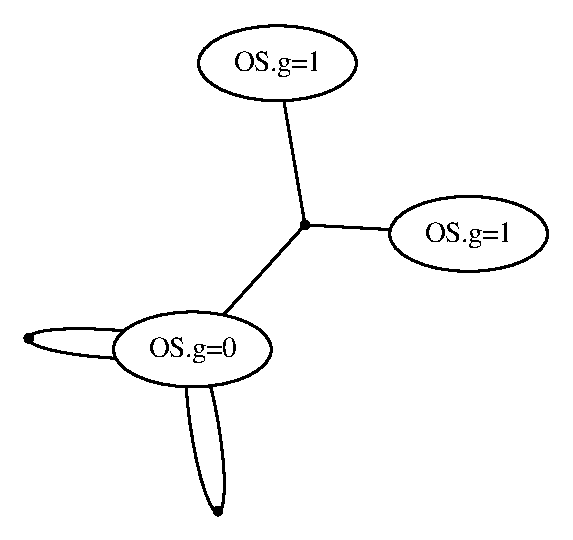
\includegraphics[width=0.55\textwidth]{figs/gluinggraph}
    \caption{Example of a gluing graph}
    \label{ch4:fig:gluinggraph}
\end{figure}

\begin{table}[ht]
\centering
\begin{tabular}{lp{4.5cm}}
    \textbf{module} & \textbf{types and functions}
    \\[4pt]
    \text{\tt SimplicialComplex} & \ensuremath{\Conid{Vertex}}, \ensuremath{\Conid{Simplex}}, \ensuremath{\Conid{Complex}},   \newline
                          \ensuremath{\Varid{connectedComponents}},            \newline
                          \ensuremath{\Varid{dfsSimplices}},                   \newline
                          \ensuremath{\Varid{parentSimplices}}
    \\[3pt]
    \text{\tt TwoDimPseudoManifold} & \ensuremath{\Varid{baseSurfaces}},            \newline
                             \ensuremath{\Varid{fixSingularity}} etc.,     \newline
                             \ensuremath{\Varid{fixAllSingularities}},     \newline
                             \ensuremath{\Varid{starSummands}} etc.
    \\[3pt]
    \text{\tt TwoDimManifold} & \ensuremath{\Varid{identifySurface}}
    \\[3pt]
    \text{\tt Surface} & \ensuremath{\Conid{Surface}}
    \\[3pt]
    \text{\tt TwoDimPseudoManifold\char46{}GluingGraph}
        \hspace*{0.8cm}                 & \ensuremath{\Conid{GluedD}} etc.,           \newline
                                          \ensuremath{\Varid{gluingGraph}} etc.       \newline
                                          \ensuremath{\Varid{gluingGraphSurf}} etc.
    \\[3pt]
    \text{\tt TwoDimPseudoManifold\char46{}GraphViz} & \ensuremath{\Varid{writeGluingGraph}},       \newline
                                      \ensuremath{\Varid{visualizeGluingGraph}}
\end{tabular}
\caption{Correspondence between presented functions and modules}
\label{ch4:tab:funcs1}
\end{table}


\section{Loop Agreement Tasks on Two-dimensional Pseudomanifolds}
\label{ch4:sec:latonpmfd}
Lastly, we consider loop agreement tasks on finite weak $2$-pseudomanifolds.
We show that the \emph{word problem} for fundamental groups of such $2$-pseudomanifolds
is solvable and use this fact in conjunction with \cref{ch3:classification}
to formulate a result about loop agreement tasks.

It is well known that the word problem for fundamental groups of closed surfaces
is solved by \emph{Dehn's Algorithm}, see
Stillwell~\cite[Sec.~6.1]{bookc:stillwell93}.
Then the following proposition is a consequence of this fact and
\cref{ch4:pmfdclass}.

\begin{thProposition}[solvability of the word problem for %
                      finite weak $2$-pseudomanifold]
    \label{ch4:wordproblem}
    %
    The word problem for the fundamental group of a $2$-dimensional finite weak
    pseudo\-manifold (based at any vertex) is solvable.
\end{thProposition}

\begin{proofsketch}
    First, observe that for finite weak $2$-pseudomanifolds $K,K'$ and vertices
    $v,v'$ of $K$ and $K'$, respectively, we have 
    \[  \pi_1\bigl( (K,v) \topowedge (K',v') \bigr)
            \cong \pi_1(K,v) \ast \pi_1(K',v')
    \]
    by the Seifert-van-Kampen theorem (where the wedge of complexes is defined
    in the obvious way). Secondly, let $K$ be a finite weak $2$-pseudomanifold
    and let $v_1,v_2$ be vertices of $K$ that have disjoint stars.
    Let $K'$ be the resulting complex after identifying $v_1$ and $v_2$ to a
    single vertex $v'$. Then we have
    \[ \pi_1(K',v') \cong \pi_1(K,v_1) \ast \Z , \]
    as can be seen by using the standard construction of the fundamental group
    of a simplicial complex in terms of generators and relations (see e.\,g.
    Herlihy~et~al.~\cite[Subsec.~15.1.2]{bookc:herlihyetal13}
    for the latter).

    Now let $K$ be a finite weak $2$-pseudomanifold, let $v\in V(K)$
    and assume without loss of generality that $K$ is connected.
    By \cref{ch4:pmfdclass} and an inductive application of the above arguments
    we see that $\pi_1(K,v)$ is isomorphic to a free product of the form
    \[ \pi_1(S_1,x_1) \ast \cdots \ast \pi_1(S_k,x_k)
        \ast \underbrace{\Z \ast \cdots \ast \Z}_{\ell\text{ times}}
    \]
    where $S_1,\dots,S_k$ are the closed surfaces that can be glued to~$K$
    \pcref{ch4:pmfdclass}, $x_j\in S_j$ for all $j\in\setOneto k$, and
    $\ell\in\N$. Now let $g_1g_2\dots g_r$ be a word in this free product.
    We apply Dehn's algorithm to each $g_j$ that is an
    element of one of the fundamental groups of the surfaces and
    freely reduce the resulting word. Then we repeat this steps until we
    either arrive at the empty word or the word cannot be reduced further.
    (This process must terminate becase the word length decreases with every
    step.) In the first case the word $g_1g_2\dots g_r$ is the identity element
    and in the second case it is non-trivial.
    \\
\end{proofsketch}

\begin{thCorollary}[loop agreement tasks on finite weak 2-pseudomanifolds]
    \label{ch4:latonpmfd}
    %
    Let $K,L\in\finSimp$ and let $\kappa,\lambda$ be triangle loops in $K$ and
    $L$, respectively. Furthermore, let $K$ and $L$ be weak $2$-pseudomanifolds.
    \begin{itemize}
        \item 
            It is decidable whether $\gamma_\kappa$ and $\gamma_\lambda$
            are (pointed) contractible in $\geom{K}$ and $\geom{L}$,
            respectively.
            
        \item
            If $\gamma_\kappa$ is (pointed) contractible,
            it is decidable whether $\Loop{K,\kappa}$ implements $\Loop{L,\lambda}$.
    \end{itemize}
\end{thCorollary}

\begin{proof}
    The first part is immediate from \cref{ch4:wordproblem}. For the second
    part let $\gamma_\kappa$ be pointed  contractible. As a direct consequence, the
    algebraic signature of~$\Loop{K,\kappa}$ is
    \[ (\pi_1(K,\dot\kappa), 1) \]
    (where $1\in\pi_1(K,\dot\kappa)$ denotes the identity element).
    Then \cref{ch3:classification}, the fact that $1$ must be mapped to the
    identity element of~$\pi_1(L,\dot\lambda)$ by any group homomorphism
    $\pi_1(K,\dot\kappa)\to\pi_1(L,\dot\lambda)$, and the first part imply
    the assertion.
    \\
\end{proof}

\medskip
Our Haskell library (see \cref{ch4:sec:implementation}) also includes a
counterpart to the theoretical \cref{ch4:latonpmfd}, that is we provide
a function\begin{hscode}\SaveRestoreHook
\column{B}{@{}>{\hspre}l<{\hspost}@{}}%
\column{4}{@{}>{\hspre}l<{\hspost}@{}}%
\column{E}{@{}>{\hspre}l<{\hspost}@{}}%
\>[4]{}\Varid{isTrivial}\mathbin{::}(\Conid{Eq}\;\Varid{a})\Rightarrow \Conid{Loop}\;\Varid{a}\to \Conid{Complex}\;\Varid{a}\to \Conid{Bool}{}\<[E]%
\ColumnHook
\end{hscode}\resethooks
that tests whether a given loop is contractible on a finite weak
$2$-pseudomanifold. Here a loop is specified as a walk \ensuremath{[\mskip1.5mu \Conid{Vertex}\;\Varid{a}\mskip1.5mu]} 
\pcref{ch3:def:walkpathcycle} with identical first and last vertex.
(Note that we also permit repeated vertices in this case.)
The main difficulty in implementing \ensuremath{\Varid{isTrivial}} is that we have
to find a representation of the loop in terms of generators and relations
in order to apply the algorithm for solving the word problem. Therefore,
the function has to trace the given loop through the process of building
the fundamental polygon and normalizing it afterwards (as mentioned in the
previous section). Since this is a rather complex procedure, we make no attempt
to explain the corresponding functions \ensuremath{\Varid{schemesWL}} and \ensuremath{\Varid{normalize}}
in detail here. After applying those functions, we get an intermediate
result of type \begin{hscode}\SaveRestoreHook
\column{B}{@{}>{\hspre}l<{\hspost}@{}}%
\column{3}{@{}>{\hspre}l<{\hspost}@{}}%
\column{E}{@{}>{\hspre}l<{\hspost}@{}}%
\>[3]{}(\Conid{GluedObj}\;\Conid{Scheme},\Conid{LoopS}){}\<[E]%
\ColumnHook
\end{hscode}\resethooks
where a \ensuremath{\Conid{Scheme}} is just a labelling scheme of a polygon, \ensuremath{\Conid{GluedObj}\;\Conid{Scheme}}
stores the schemes for our surfaces~$S_j$ (of \cref{ch4:pmfdclass})
and a \ensuremath{\Conid{LoopS}} is a representation of our input loop in terms of the symbols
used in those schemes.
As an example, consider the wedge of two tori. Then the first component of the
above tuple would contain the labelling schemes $aba^{-1}b^{-1}$ and
$cdc^{-1}d^{-1}$ and the second component would be any word in the letters
$\{a,b,c,d\}$ and their formal inverses. For instance,
$abcdc^{-1}d^{-1}a^{-1}b^{-1}$ would specify a contractible loop.

The last step is the implementation of \cref{ch4:wordproblem}. The function\begin{hscode}\SaveRestoreHook
\column{B}{@{}>{\hspre}l<{\hspost}@{}}%
\column{3}{@{}>{\hspre}l<{\hspost}@{}}%
\column{E}{@{}>{\hspre}l<{\hspost}@{}}%
\>[3]{}\Varid{simplifyLoop}\mathbin{::}\Conid{GluedObj}\;\Conid{Scheme}\to \Conid{LoopS}\to \Conid{LoopS}{}\<[E]%
\ColumnHook
\end{hscode}\resethooks
takes the data described in the last paragraph and reduces the loop to either
the empty word (in which case the input loop is in fact contractible) or a
word that cannot be further simplified. Depending on the involved surfaces
\ensuremath{\Varid{simplifyLoop}} uses the functions \ensuremath{\Varid{simplifyOnX}} (with \ensuremath{\Conid{X}} one of
$\{\text{\ensuremath{\Conid{Sphere}}}, \text{\ensuremath{\Conid{Torus}}}, \text{\ensuremath{\Conid{PrPlane}}}, \text{\ensuremath{\Conid{KleinB}}}\}$)
and \ensuremath{\Varid{dehnAlg}} to solve the word problem.

The implementation of Dehn's algorithm and the function \ensuremath{\Varid{dehnAlg}} can be found
in the module \text{\tt DehnAlgorithm} and all other functions of this section are
defined in \text{\tt TwoDimPseudoManifold\char46{}Loop}.


\appendix
\printbibliography\newpage
\mbox{}\thispagestyle{empty}
\chapter*{Selbstständigkeitserklärung}\thispagestyle{empty}
Ich habe die Arbeit selbstständig verfasst, keine anderen als die angegebenen
Quellen und Hilfsmittel benutzt und bisher keiner anderen Prüfungsbehörde
vorgelegt. Außerdem bestätige ich hiermit, dass die vorgelegten Druckexemplare
und die vorgelegte elektronische Version der Arbeit identisch sind, dass ich
über wissenschaftlich korrektes Arbeiten und Zitieren aufgeklärt wurde und dass
ich von den in \S~26/27 Abs.~5 vorgesehenen Rechtsfolgen Kenntnis habe.

\vspace{2cm}
\noindent
\rule{4cm}{0.4pt}, den \rule{3cm}{0.4pt} \qquad \rule{6cm}{0.4pt}



\end{document}

